% !TEX TS-program = XeLaTeX
%************************************************
\chapter{Solubility of Radon Daughters in Liquid Xenon}\label{ch:radon} % $\mathbb{ZNR}$
%************************************************
Rare-event searches are very sensitive to backgrounds from radioactivity in and on detector materials. Some of the most omnipresent and troublesome are $^{222}$Rn and its daughters. Decay products from $^{222}$Rn plate out on detector surfaces and have typically been assumed to be fixed there. In this chapter, a series of experiments is described; the results provide evidence that radon daughters can dissolve in liquid xenon.

\section{Motivation}
Radon and radon daughters produce problematic backgrounds for rare-event searches \cite{LUXFirstResults}. Of particular concern for liquid xenon dark matter detectors are ``naked'' beta decays. These ground-state to ground-state decays have no accompanying gammas and cannot be rejected via coincidence tagging. Rejection of these backgrounds in WIMP search experiments relies solely on being able to discriminate electron recoils from nuclear recoils. For example, the \ac{ER} leakage fraction from the LUX Run03 tritium calibration is on the order of 2/1000 over the WIMP search region \cite{LUX:Tritium} (See Chapter ?? for more details).  The $^{222}$Rn chain contains $^{210}$Pb ($T_{1/2} = $~22.23~y), effectively splitting the decay chain into a ``fast chain'' and ``slow chain'' (Fig. $\ref{fig:Rn222}$). Radon can be introduced via two pathways: (1) during detector construction and (2) during detector operation (see Fig. $\ref{fig:flow_chart}$). Great care is taken to ensure minimal contamination via pathway 2 because the fast chain naked betas, $^{214}$Pb and $^{214}$Bi, may decay in the fiducial volume before the purification system can remove them or before they can plate out on detector surfaces. In pathway 1, $^{222}$Rn and daughters plate out onto detector surfaces during construction of parts, and construction of the detector itself. Models for plate out can be found in \cite{Guiseppe:2011mj} and \cite{Knutson:1988}. Typically it is assumed that once $^{222}$Rn and daughters plate out, they remain fixed at that position, and can be rejected by a fiducial volume cut. This means that the slow chain naked betas of $^{210}$Pb and $^{210}$Bi from initial exposure during construction are assumed to occur outside the fiducial volume. However, evidence of $^{210}$Bi mobility has been observed in the liquid scintillator environment of KamLAND  \cite{Takemoto:2015gta}, \cite{Gando:2014wjd} and Borexino \cite{Bellini:2013lnn}. If radon daughters are soluble in liquid xenon, the late chain naked betas (from both pathway 1 and 2) pose a serious background distributed throughout the fiducial volume.


\begin{figure}[ht]
    \centering
    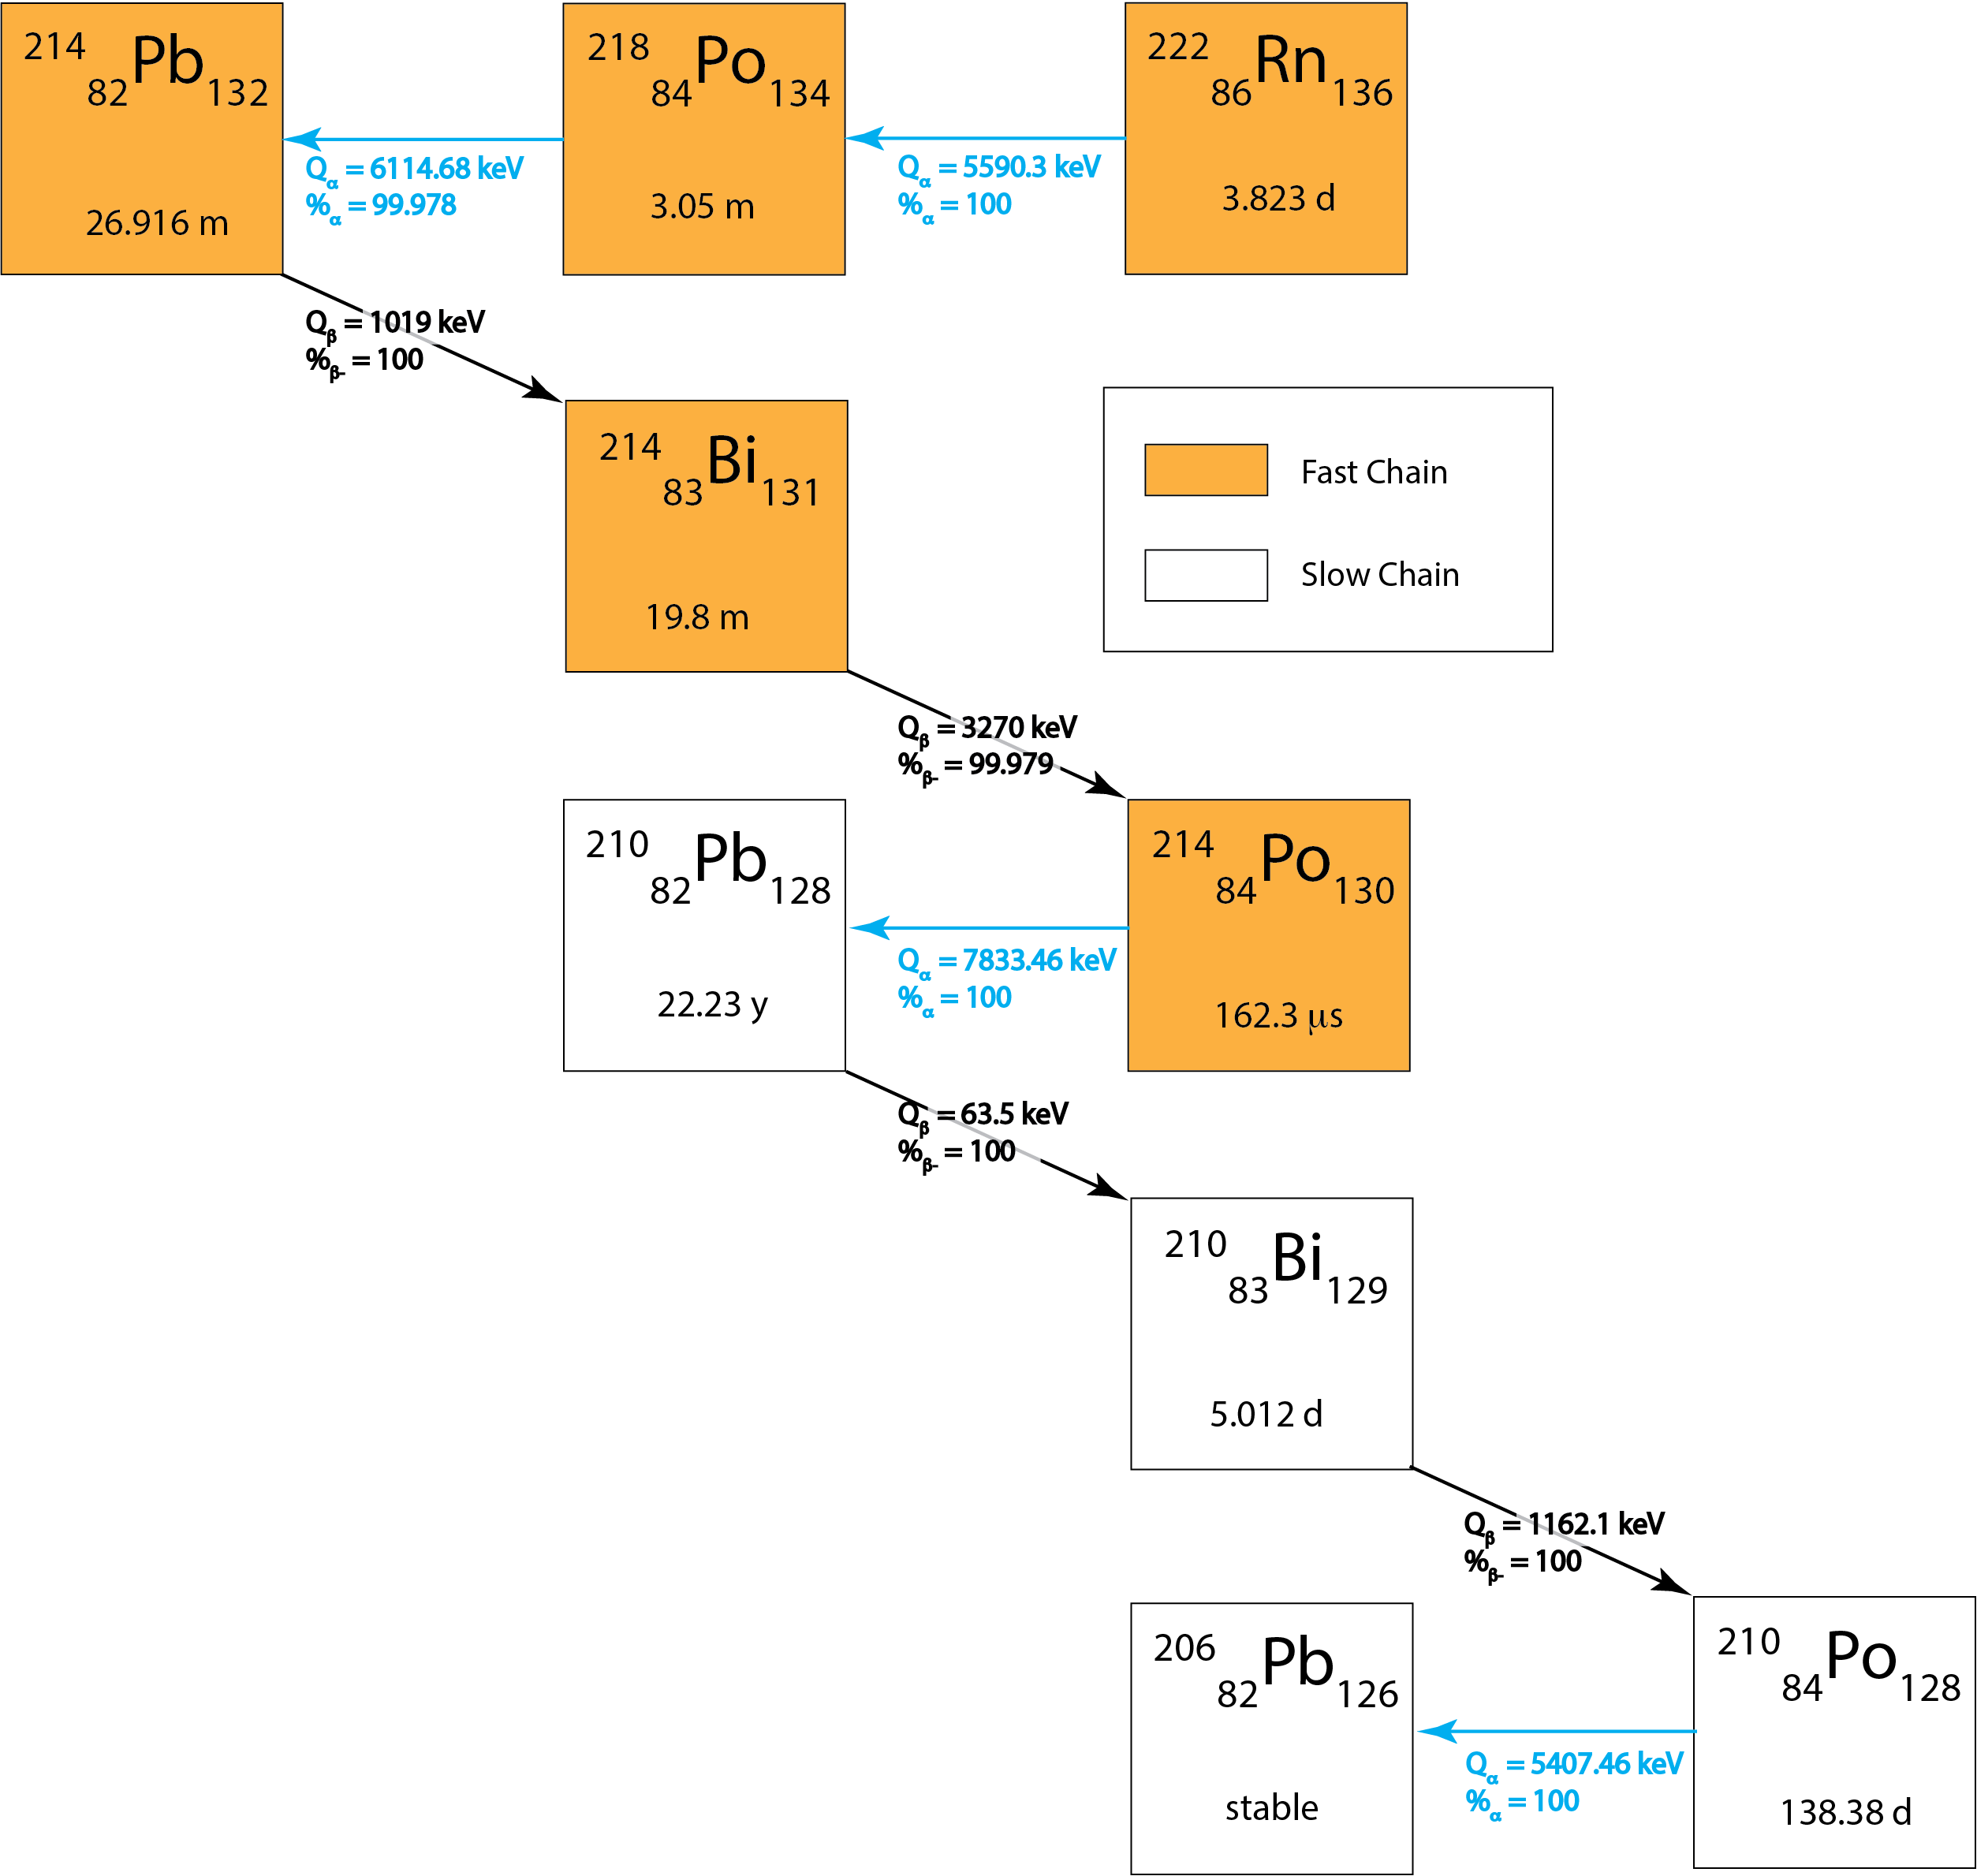
\includegraphics[width=5.0in]{figures/radon/222Rn_simple_fastslowchains.png}
    \caption{The $^{222}$Rn decay scheme. The fast and slow chains are indicated.}
    \label{fig:Rn222}
\end{figure}

\begin{figure}[ht]
    \centering
    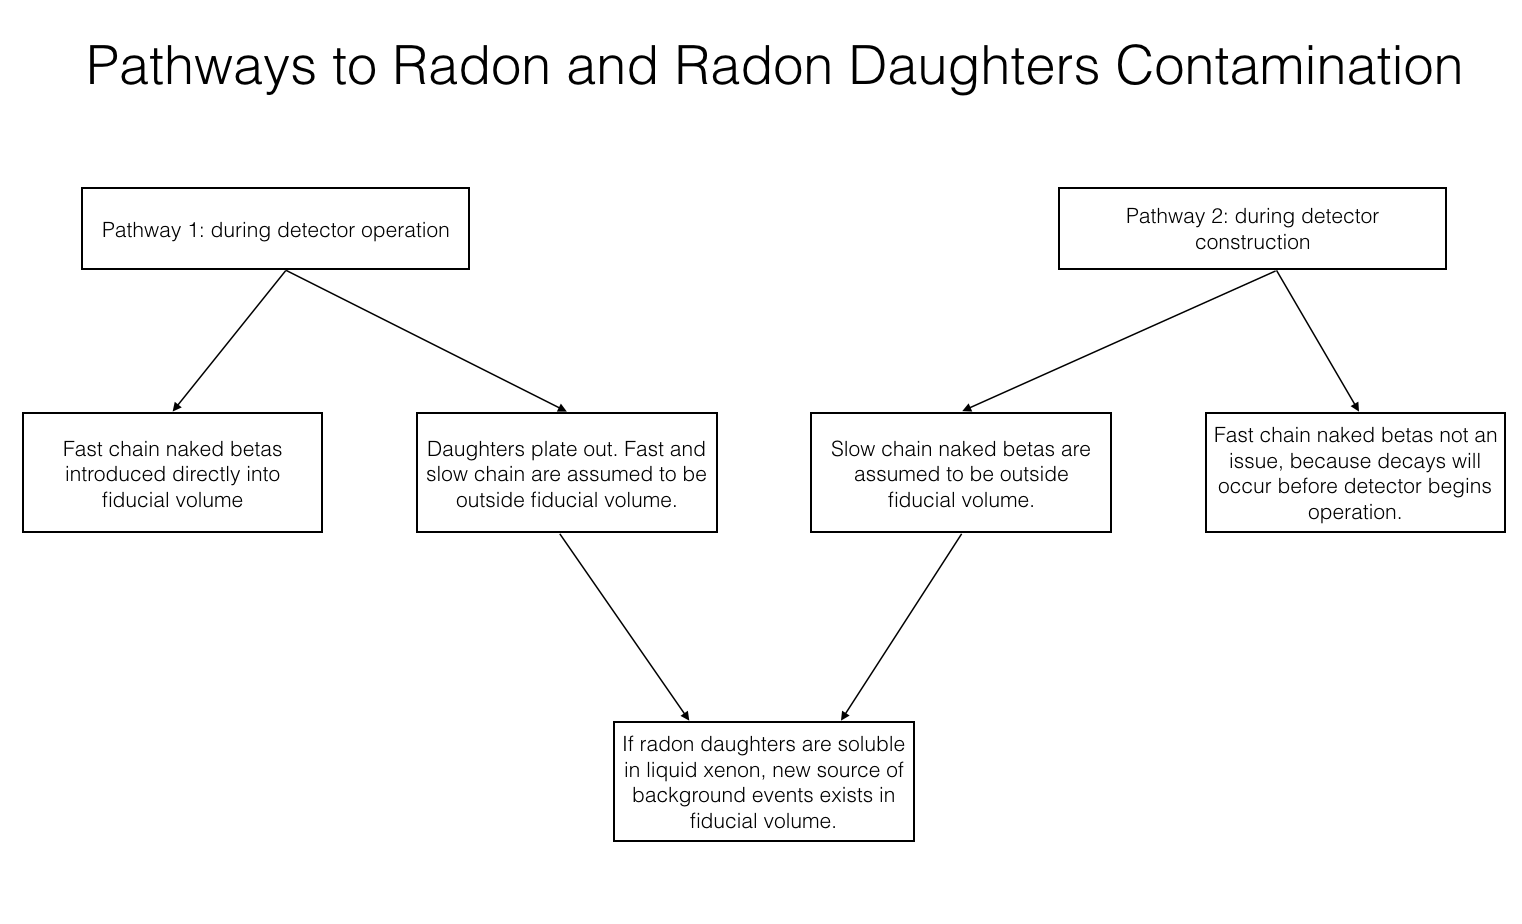
\includegraphics[width=6.0in]{figures/radon/Rn_pathways.png}
    \caption{Pathways to radon and radon daughter contamination.}
    \label{fig:flow_chart}
\end{figure}


%While $^{222}$Rn has a half-life of 3.8~d, the long-lived daughter $^{210}$Pb ($T_{1/2} \approx$~22.3~y) can be a source of background events in even the longest running searches. Of particular concern for liquid xenon dark matter detectors are the ``naked'' beta decays of $^{210}$Pb and $^{210}$Bi. These ground-state to ground-state decays have no accompanying gammas and cannot be rejected via coincidence tagging. Rejection of these backgrounds in WIMP search experiments relies solely on being able to discriminate electron recoils from nuclear recoils. Typically it is assumed that once $^{222}$Rn and daughters plate out, they remain stuck to the surface, and can be rejected by a fiducial volume cut. However, evidence of $^{210}$Bi mobility has been observed in the liquid scintillator environment of KamLAND  \cite{Takemoto:2015gta}, \cite{Gando:2014wjd} and Borexino \cite{Bellini:2013lnn}. If radon daughters are soluble in liquid xenon, the naked beta decays of $^{210}$Pb and $^{210}$Bi pose a serious background distributed throughout the fiducial volume.

In order to investigate the solubility of radon daughters in liquid xenon, a $^{220}$Rn source was employed. The analogous long lived daughter in this chain, $^{212}$Pb, has a half-life of 10.6~h, making it appropriate for a laboratory test. Investigating pathway 2 in the laboratory by introducing radon in a \ac{LXe} environment will necessarily yield inconclusive results, because it is impossible to tell if the daughter decay of interest plated out before decaying. Therefore, we required the radon daughters to be on a surface.

Xenon gas was circulated through the $^{220}$Rn source and detector components for a period of $>$24~h. The detector was then evacuated, thereby assuring the initial position of radon daughters on a detector surface. Any radon daughters subsequently observed in the bulk region after condensing liquid xenon must therefore have dissolved.

%There are two main pathways to radon contamination for rare-event searches with liquid xenon time projection chambers (LXe TPCs):

%1. During construction, radon plates out onto detector surfaces. This radon and subsequent daughters are assumed to remain stuck in a liquid xenon environment.

%2. During operation, radon that emanates into the detector volume decays wherever it is deposited by circulation and/or convection currents. In LXe TPCs, a drift field in the large bulk region drifts the 75\% of charged radon daughters towards the bottom of the detector, where they are then assumed to remain. The radon daughters that are not charged remain in the bulk region, where they then have the chance to be removed by the detector purification system. 

%Testing pathway 2 by depositing radon into a liquid xenon environment will yield inconclusive results. A radon daughter decay purposely deposited in the bulk cannot be distinguished from a radon daughter which dissolved into the liquid after plating out at the bottom of the detector. Therefore, we focus on pathway 1 by only introducing radon in a gas environment, thereby assuring its initial position on a detector surface. Then any radon daughters observed in the bulk region after condensing liquid xenon are candidates for having dissolved.
%tentative statement: testing pathway \#2 is always going to be inconclusive because ... therefore we focus on pathway \#1.

\subsection{Plate Out}
The term ``plate out'' is used above but not defined. The literature indicates that there two known types of radon daughter plate out \cite{Samuelsson1996}. The following terms are used in  \cite{Samuelsson1996} to identify each type.

\begin{enumerate}
\item \textit{implantation} Alpha recoil implantation of a daughter nucleus
\item \textit{sticking} Daughters are sitting on the surface of a material, it is possible to wash a percentage of these off with various surface cleaning methods.
\end{enumerate}

The percentages of daughters plated out in these different modes are not indicated, but \cite{Samuelsson1996} relates a story of researchers being unable to remove $^{214}$Po from glass samples, where as $^{218}$Po was easily removed with surface cleaning methods. This is explained by the fact that further down the $^{222}$Rn chain, more alpha decays have occurred, so a late-state daughter has had more changed to be implanted. It is also noted that the  durability of the implanted activity subject to change under different conditions, as is the implant integrity. The author cites factors such as humidity and temperature affecting whether daughters implant, and whether they remain implanted; since the conditions for plate out are different in pathways 1 and 2 and it logical to infer that implantation functions differently in these two environments for \ac{LXe} \ac{TPC}s. 

The chemistry of radon has been studied as well, and may provide some context to the plate-out discussion. Radon is frequently regarded as a totally inert element. It is, however, classified as a ``metalloid", and exhibits some of the characteristics of both true metals and nonmetals. For example, it is known to react chemically with fluorine, halogen fluorides, dioxygenyl salts, fluoro-nitrogen salts, and halogen fluoride-metal fluoride complexes to form ionic compounds \cite{stein1982}. It is also known to co-crystalize with hydrogen chloride, hydrogen sulfide, sulfur dioxide and carbon dioxide \cite{stein1987}. In the latter case, the author notes that the radon is not forming true chemical bonds, but rather is held in place by weak Van der Waals forces. These chemical experiments found radon to be readily reactive at ``room temperature and lower", but the low temperate range is not stated. Chemical bonds formed by radon may make up a different type of plate out, or sub-type of `sticking'. Presumably weak surface Van der Waals forces belong in the `sticking' type as well. 

If we look to surface physics, the plate-out term `sticking' is well defined by the terms physisorption and chemisorption. Physisorption is distinct from chemisorption in that it is a general phenomenon occurring between the adsorbed atom and surface, where chemisorption involves a chemical reaction between surface and adsorbate, and is characterized by higher bond strengths. Chemisorption potentials have been calculated for many atoms and surfaces \cite{HammerNorskov} and are generally greater than 1~eV. Physisorption potentials, such as the well-known Van der Waals potential, are less than 1~eV and as low as 10~meV. 


Plate out occurs with different rates on different materials \cite{Bigu1987}, and can be an order of magnitude larger on PTFE than stainless steel, likely due to PTFE's tendency to accumulate negative static charge \cite{Morrison2017}. Plate out of radon daughters can be reduced by employing a nitrogen gas purge or an electric field (approximately 90\% of radon daughters are charged) \cite{Bruemmer2015}. However, \cite{Bigu1987}, \cite{Morrison2017}, and \cite{Bruemmer2015} do not distinguish between implantation and sticking, and only use the term ``plate out''. 


\section{Experimental Configuration and Method}
\begin{figure}[ht]
    \centering
    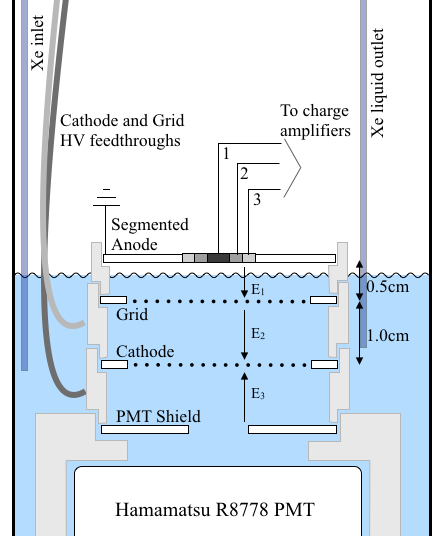
\includegraphics[width=3.0in]{figures/radon/internals.png}
    \caption{Diagram of the test bed. For this study, the cathode is held at -6.0 kV, and the grid is held at -4.0 kV. E$_{1}^{liq} \approx $5.0 kV/cm, E$_{1}^{gas} \approx $10.0 kV/cm E$_{2}$ = 1.0 kV/cm. E$_{3}$ = 2.7 kV/cm. The large gray regions represent the structural rings of PTFE. The line between the grid and anode represents the liquid xenon level. The xenon inlet pipes incoming gas directly into the liquid region, and the liquid outlet pulls from the level of the active region. A gas outlet (not pictured) also draws xenon gas into the circulation system to be purified.}
    \label{fig:anode_and_grids}
\end{figure}

A diagram of the TPC for this work is shown in Fig. $\ref{fig:anode_and_grids}$. A 50~mm diameter cathode wire grid, extraction wire grid, and a planar, segmented anode were held in Teflon PTFE housing. The anode was instrumented with charge-sensitive preamplifiers. Both grids were constructed from a stainless steel frame strung with 4~$\mu$m diameter stainless steel wire on a 2~mm pitch. The xenon inlet was a PTFE tube which introduced xenon gas into the liquid region where it was condensed. The xenon liquid outlet was a thin stainless steel capillary that drew liquid from the TPC into the purification system. Both inlet and outlet tubes were placed near holes drilled in the PTFE to aid circulation into the active volume.

A particle interaction in the liquid xenon volume produced primary scintillation photons (S1) and ionization electrons. The ionization electrons were drifted with an electric field into the gas phase, where they produced secondary scintillation light (S2). A single Hamamatsu R8778 VUV-sensitive PMT was installed in Teflon PTFE housing, facing upward to view the active region. Directly above the PMT was a copper shield mask, held at the same voltage as the PMT bias of -1250~V.

%During data-taking, the cathode, grid, and anode were were held at -6.0~kV, -4.0~kV, and 0~V, respectively. 


%A cathode wire grid was held in place 1~cm above the PMT shield. An extraction wire grid was held 1~cm above the cathode grid. A planar, segmented anode was held 0.5~cm above the extraction grid and instrumented with charge-sensitive preamplifiers. Both grids were constructed from a stainless steel frame strung with 4~$\mu$m diameter stainless steel wire on a 2mm pitch. 


%The Cirlex {\color{red} [it is made of G10]} anode has three segments, which directly measure charge. Each segment is read out via a charge-sensitive preamplifier. The readout segments are concentric: channel 1 is the central circle, channel 2 is the ring around it, and channel 3 is the outermost ring. The extraction grid has the dual purpose of creating a higher field than the drift region to extract electrons into the gas region of the TPC, as well as being used as a Frisch grid to reduce the z-dependence of charge measurement. The voltage of the extraction grid relative to the cathode is determined by Bunneman's equation for grid transparency (Ref here?).

%An outer stainless steel vessel surrounding the TPC is kept at vacuum.

The TPC was filled with 1.5~bar of xenon gas at room temperature. The gas was circulated continuously through the TPC and a heated zirconium getter for at least 24 hours to remove contaminants. The TPC was then cooled to $-100^{\circ}$~C while circulating xenon gas. Circulation was stopped, and xenon was condensed into the TPC until the liquid level rose to between the extraction grid and anode. The process of filling the TPC took 4 to 5 hours. The liquid level was kept stable by keeping the temperature and pressure constant in the TPC. During data collection, xenon from the TPC was circulated through a getter and re-condensed into the TPC to remove impurities. %A capillary circulates xenon from the liquid region and an additional, separate valve circulates gaseous xenon from column of gas above the active region to prevent stagnation. This circulation line bypasses an $^{220}$Rn flow-through source. If desired, the flow can be switched from the bypass line to the source, bringing $^{220}$Rn into the TPC. The circulation path is through the source during plate-out, described below, and through the bypass during data-taking. 

\begin{figure}[ht]
    \centering
    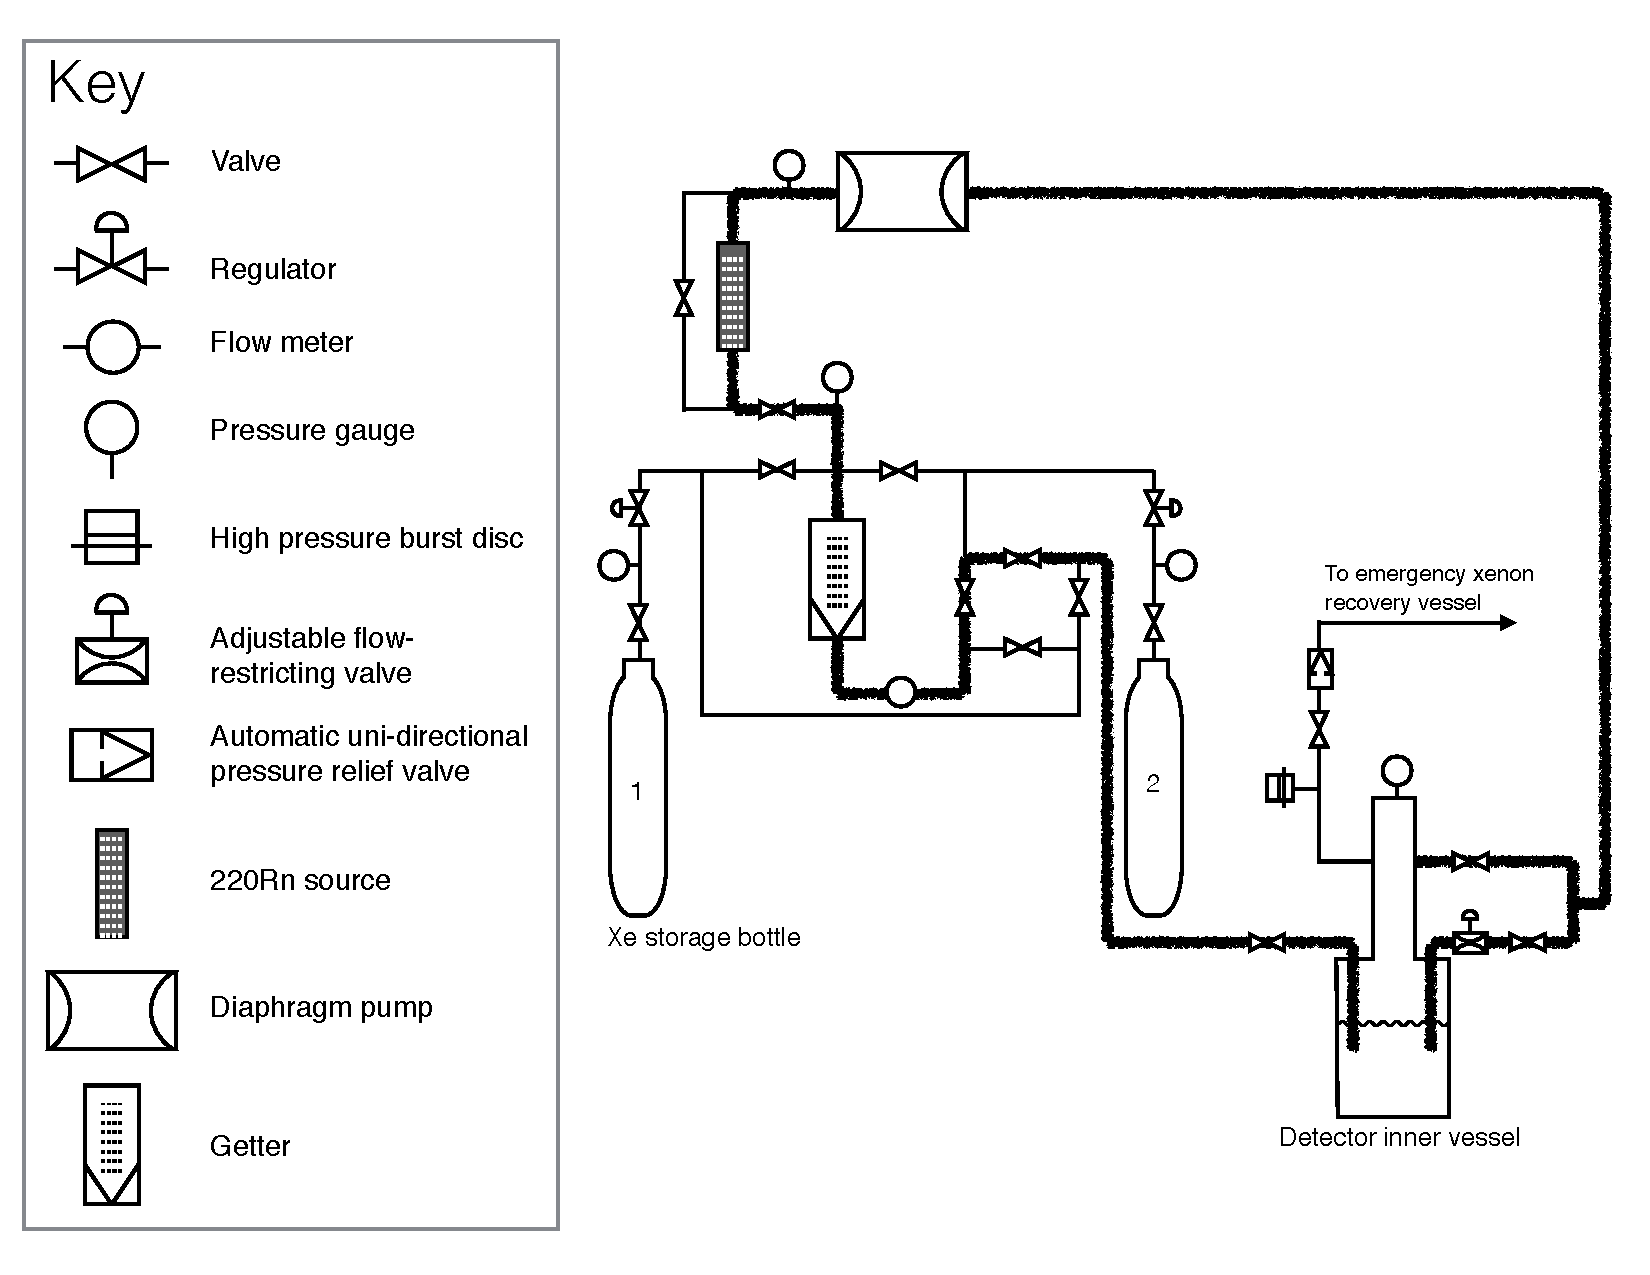
\includegraphics[width=5.0in]{figures/radon/Rn_Circulation_Path.pdf}
    \caption{An example a circulation path used for plate out is shown on the pumping and instrumentation diagram. During data-taking the radon source was bypassed. The typical liquid level is indicated on the diagram to show that the outlet drew from the liquid via a capillary, ensuring purification of the liquid xenon. A gas purge also purified the gas column in the detector.}
    \label{fig:p_and_id}
\end{figure}

\subsection{Plate Out of $^{220}$Rn Daughters}
\label{plateout}
The procedure to plate out $^{220}$Rn daughters on the inner surfaces of the detector was the same as described in Sec. $\ref{procedure}$, except that the circulation path was directed through a 2~kBq $^{220}$Rn source. The $^{220}$Rn is shown in Fig. $\ref{fig:Rn220}$. The rate of radon activity in the TPC was measured to be $4.5\pm0.5$~Hz during plate out. The total alpha rate was measured by taking repeated 1200~ms traces on an oscilloscope of the PMT with a falling edge trigger and counting the alpha decays. This rate was then halved to get the rate of radon decays. The $4.5\pm0.5$~Hz rate of radon activity represents activity for all of the space internal to the PTFE support structure. Decay daughters diffused until they contacted a wall or other surface, where they could plate out. Some percentage of decay daughters are expected to be positively charged ions. If the cathode grid was biased, charged decay daughters drifted preferentially to the cathode grid. The cathode voltage during plate outs is noted in Table $\ref{T:1}$.

\begin{figure}[ht]
    \centering
    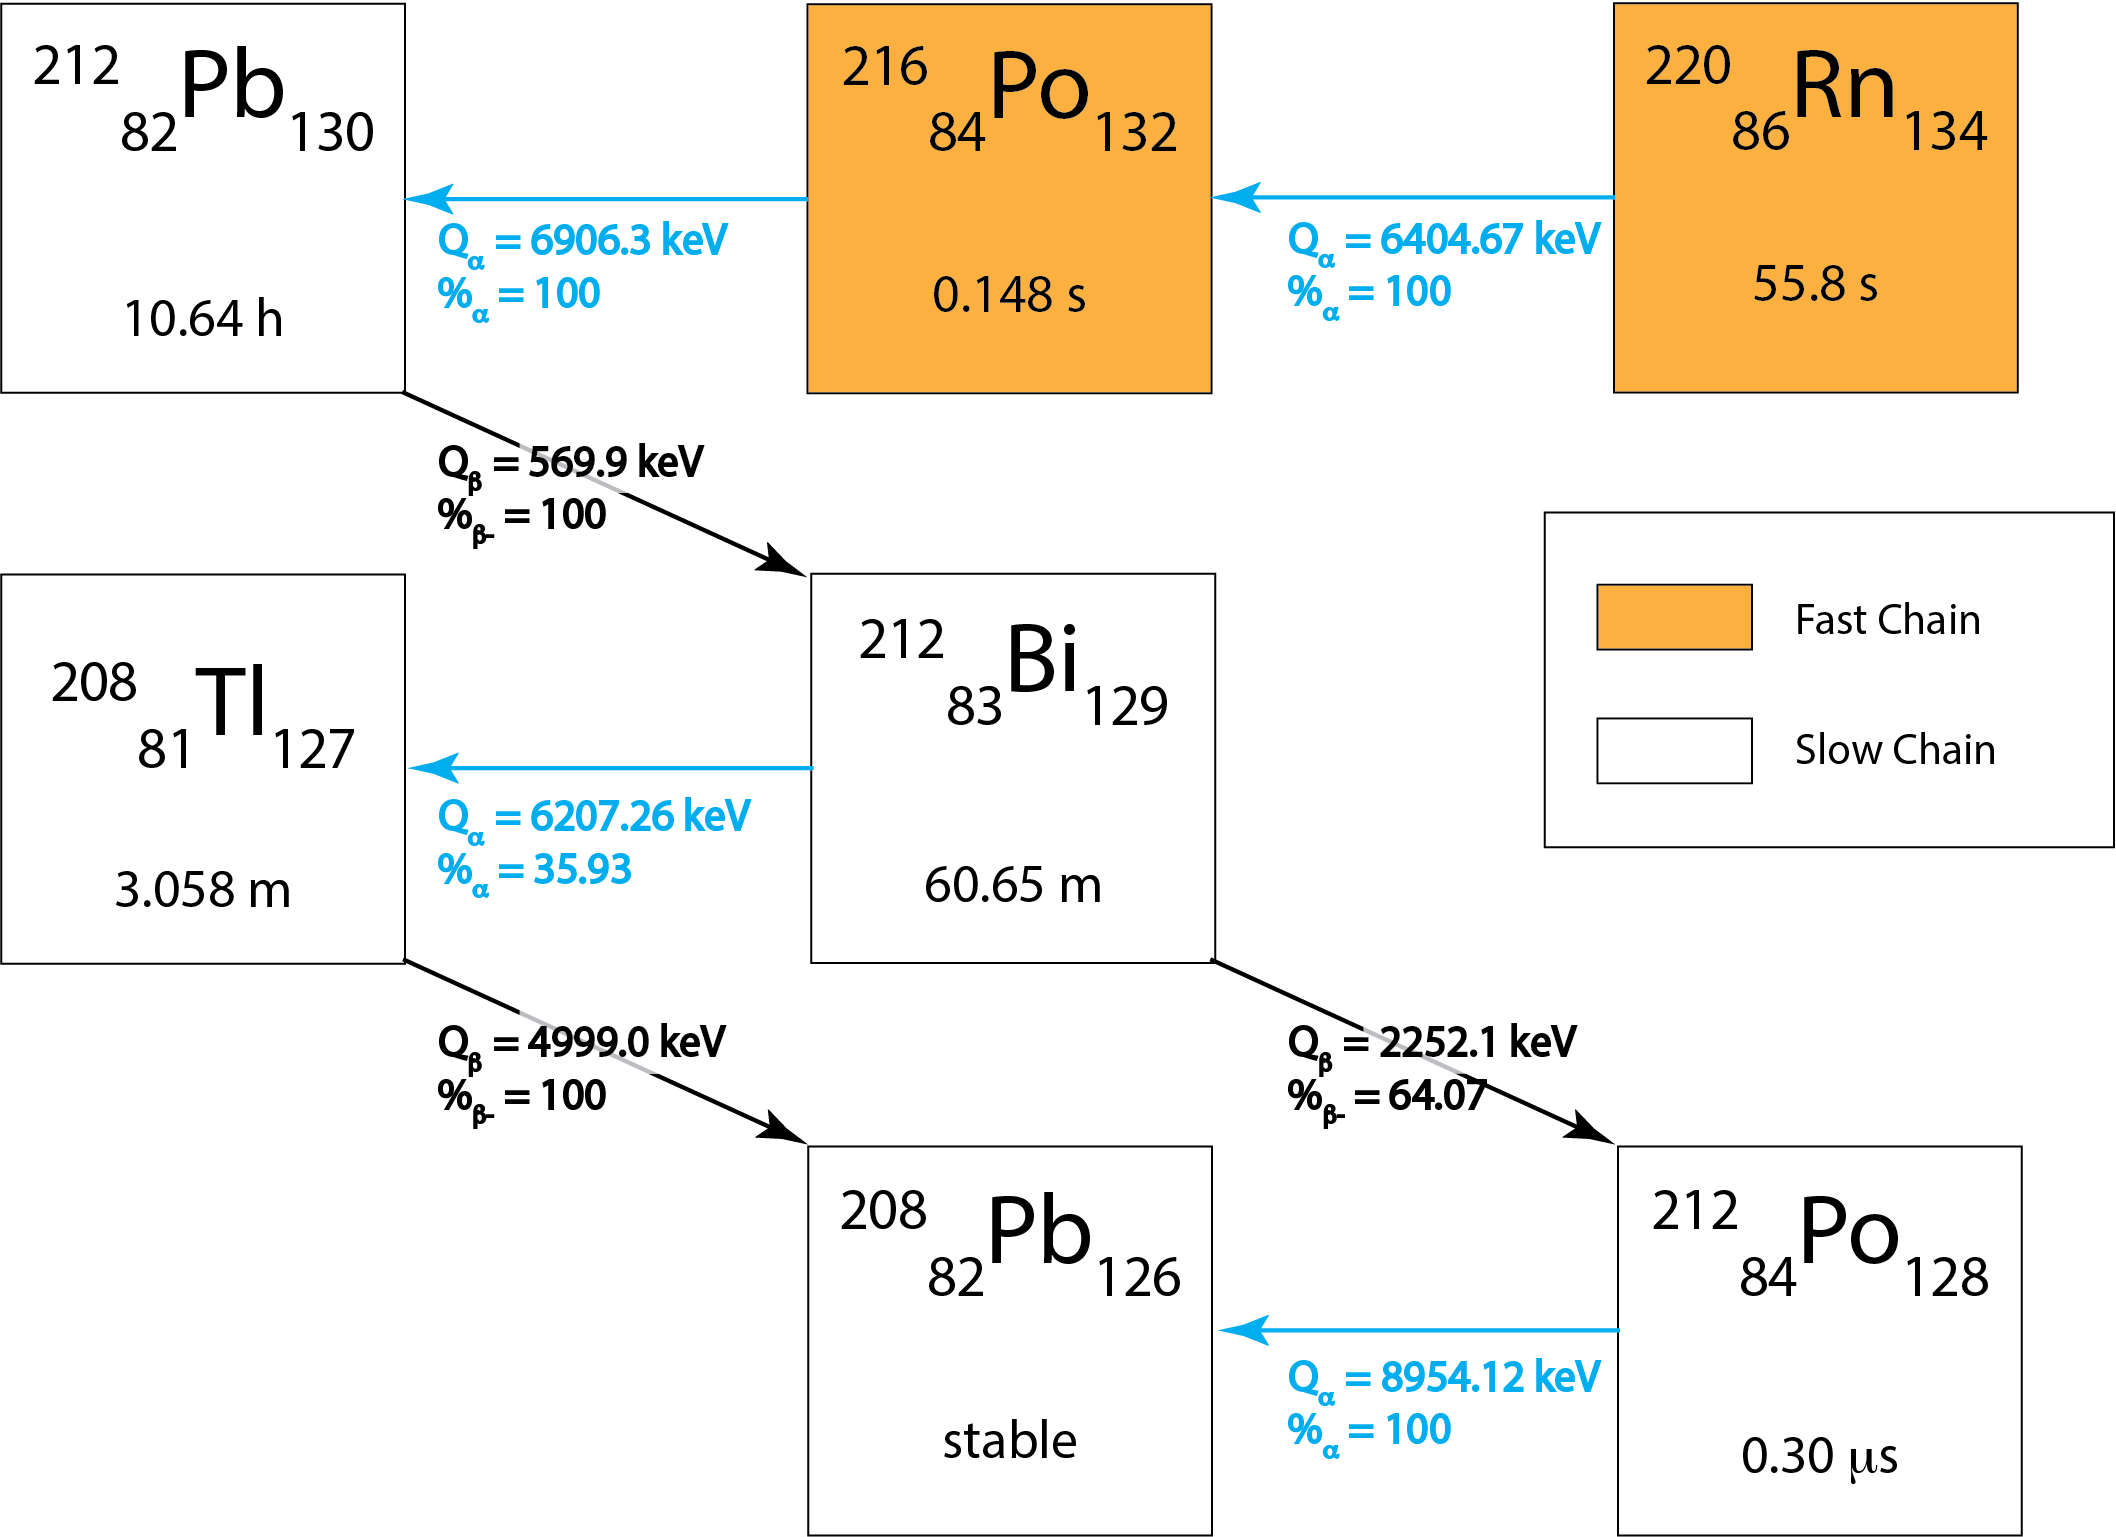
\includegraphics[width=5.0in]{figures/radon/220Rn_simple_fastslowchains.png}
    \caption{The $^{220}$Rn decay scheme. The fast and slow chains are indicated. Events in the plate out data sets are from the slow chain.}
    \label{fig:Rn220}
\end{figure}

Prior to filling the TPC with liquid xenon, the circulation was stopped and the xenon gas removed from the TPC and the circulation lines. A vacuum pressure of a few $10^{-4}$~Torr was achieved in a period of ten minutes. This step ensured removal of $^{220}$Rn and decay daughters which are dissolved in the gas, leaving only those daughters which had plated out on a detector surface. Since the fill time of the TPC is 4 to 5 hours, there were no fast chain alpha decays of $^{220}$Rn and $^{216}$Po in the plate out data. Additional details are summarized in Table $\ref{T:1}$.

\begin{table}[ht]
\centering
\begin{tabular}{llcccc}
\hline
\\[-5pt]
%& \multicolumn{3}{c}{\bf Datasets}\\[-5pt]
\\[-5pt]
& dataset ID & A &B & C & D \\
\\[-5pt]
\hline
\\[-5pt]

\multirow{3}{*}{Plate-Out} & Circ thur $^{220}$Rn Source & yes & yes & no & - \\
& Circulation Time (h) & 24 & 48 & 24 & - \\
& Cathode Voltage (kV) & -1 & 0 & 0 &  - \\
\\[-5pt]

\multirow{3}{*}{Data-Taking} & Circ thur $^{220}$Rn Source & no & no & no & yes\\
& Cathode Voltage (kV) & -6 & -6 & -6 & -6 \\
& Grid Voltage (kV) & -4 & -4 & -4 & -4 \\

\\[-5pt]
& Livetime (h) & 12.02 $\pm$ 0.5 & 23.93 $\pm$ 0.5 & 25.02 $\pm$ 0.2 & 4.15 $\pm$ 0.2  \\

%\hline
%\\[-5pt]
%\rowgroup{Run Conditions:} \\
%Livetime (hrs) & 24 & 24 & 24 \\
%Mass Xe filled (g) & 980 & 980 & 980 \\
%\\[-5pt]
%\hline
\\[-5pt]
%\rowgroup{Results:} \\
%Signal Events  & 11 & 20 & 1 \\
%Percent Dissolved & 0.3 & 0.6  & 0.03 \\
%\\[-5pt]
\hline
\end{tabular}
\caption{Summary of plate out and data-taking conditions. Data sets A and B are taken after circulating radon gas and data set C, background, had no radon circulation. Data set D was taken following dataset A, and radon was circulated in a liquid xenon environment, purposefully introducing radon into the detector bulk to calibrate the detector.}
\label{T:1}
\end{table}


\subsection{Data Collection}
\label{datacollection}
Voltage records from PMT and charge channels were collected with a 14-bit ADC with 125~MHz sampling and a 20~MHz low-pass filter. The trigger was a coincidence between the PMT and the central anode segment, used to select events in the central ($r<3$~mm) column of xenon. This avoids any electric field fringing effects. %and also minimizes any variation in S2 size f. 

\subsection{Calibration}
In order to identify a signal region for bulk radon daughters, the flow though $^{220}$Rn source was employed directly following dataset A, allowing $^{220}$Rn to flow into the liquid bulk of the TPC. The bulk daughter decay of interest, $^{212}$Bi alpha, has an energy approximately equal to the $^{220}$Rn alpha decay. The alpha signals were sufficient to saturate the biasing circuit of the PMT, so alpha decays within 1~MeV of each other were indistinguishable. Therefore, the region in S1 area vs. S2 area where the $^{220}$Rn alphas appeared was also where $^{212}$Bi alphas were expected (Fig. $\ref{fig:all_plots_CD}$).

\subsection{Position Reconstruction}
The central anode segment was assumed to select events from the central column with 100\% efficiency. Events occurring under one of the outer concentric segments can produce a signal on the central anode, but the signal was largest at the anode nearest the charge. It was not required that there be zero signal on the outer segments, so the (x,y) position of the event is treated as a source of uncertainty, which is taken into account in the calculation of fiducial volume.
The drift time of the events was calculated from the time difference between the S1 and S2 pulses, and a linear scaling of 2~mm/us was applied using the Miller (1968) electron drift velocity in \ac{LXe} measurements. 

\subsection{Fiducial Volume}
Different values for the fiducial volume are presented below.


\begin{table}[ht]
\centering
\begin{tabular}{ccccc}
\hline
\\[-5pt]
%& \multicolumn{3}{c}{\bf Datasets}\\[-5pt]
\\[-5pt]
 Anode Segments & 1 & 2 & 3 & Full \\
\\[-5pt]
\hline
\\[-5pt]
Radius (mm) & 3  & 6 & 9 & 24 \\
\\[-5pt]
Area (mm$^{2}$) & 28 &  113 & 255 & 1810 \\
\\[-5pt]
Volume (mL) & 0.39 $\pm$ 0.03 & 1.6 $\pm$ 0.1& 3.6 $\pm$ 0.3 & 25.3 $\pm$ 1.8 \\
\\[-5pt]
Mass (g) & 1.1 $\pm$ 0.1 & 4.6 $\pm$ 0.3 & 10 $\pm$ 1 & 73.4 $\pm$ 5.2  \\
\\[-5pt]

\hline
\end{tabular}
\caption{Calculations of fiducial volume. Liquid level is taken to be 14 $\pm$ 1 mm. Density of \ac{LXe} near boiling point is 2.9~g/mL.}
\label{T:fiducial}
\end{table}






\section{Analysis}
\label{S:3}
\subsection{Number of $^{220}$Rn daughters in the TPC}
As described in Sec. \ref{plateout}, the rate of $^{220}$Rn in the TPC was measured to be 4.5 $\pm$ 0.5 Hz during  plate out. From this, the number of daughter atoms $^{212}$Pb and $^{212}$Bi present in the TPC just prior to filling the liquid xenon were calculated. The number of daughter atoms as a function of the plate out time is shown in Fig. $\ref{fig:plate_out}$ along with the data acquisition periods for each dataset. This calculation assumes that the diffusion time in the PTFE walls was less than removal time via the capillary.

%, and is an upper bound because some of the daughters are swept with the gaseous xenon through the circulation system and removed by the getter, or similarly removed with the pump out step prior to data taking. There is no way to accurately estimate the number of $^{212}$Bi atoms deposited on detector surfaces, so we use the upper bound in the calculation of percent of dissolved $^{212}$Bi below.  

%\begin{figure}[hbtp]
%\centering
%\subfloat[]{\includegraphics[width=\halffig]{figures/ibl_transverse.png}}\\
%\subfloat[]{\includegraphics[width=\halffig]{figures/ibl_longitudinal.png}}
%\caption{A three-dimensional computer-generated image of the geometry of the \acs*{IBL} with a view (a) mostly transverse to the beam pipe (b) mostly parallel to the beam pipe~\cite{ibl_tdr}.}
%\label{fig:ibl_geometry}
%\end{figure}



\begin{figure}[hbtp]
\centering
\subfloat[]{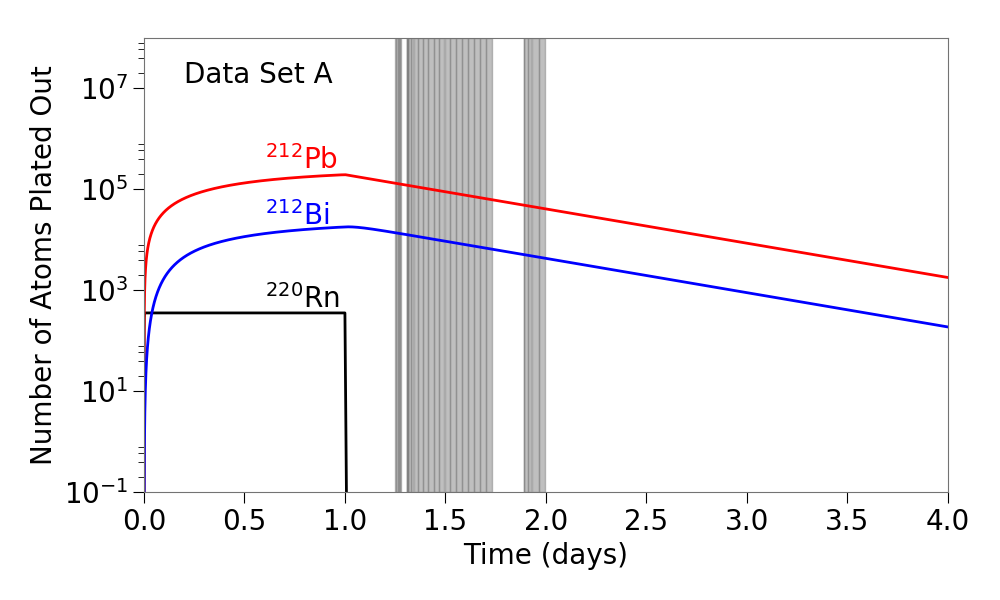
\includegraphics[width=\fullfig]{figures/radon/livetime_a.png}}\\
\subfloat[]{ 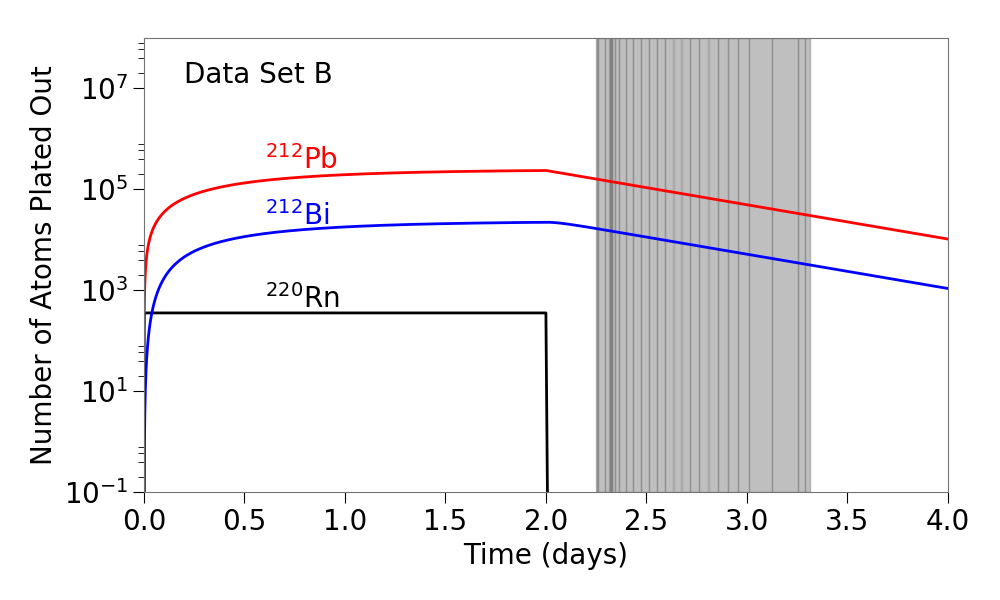
\includegraphics[width=\fullfig]{figures/radon/livetime_b.png}}\\
\subfloat[]{   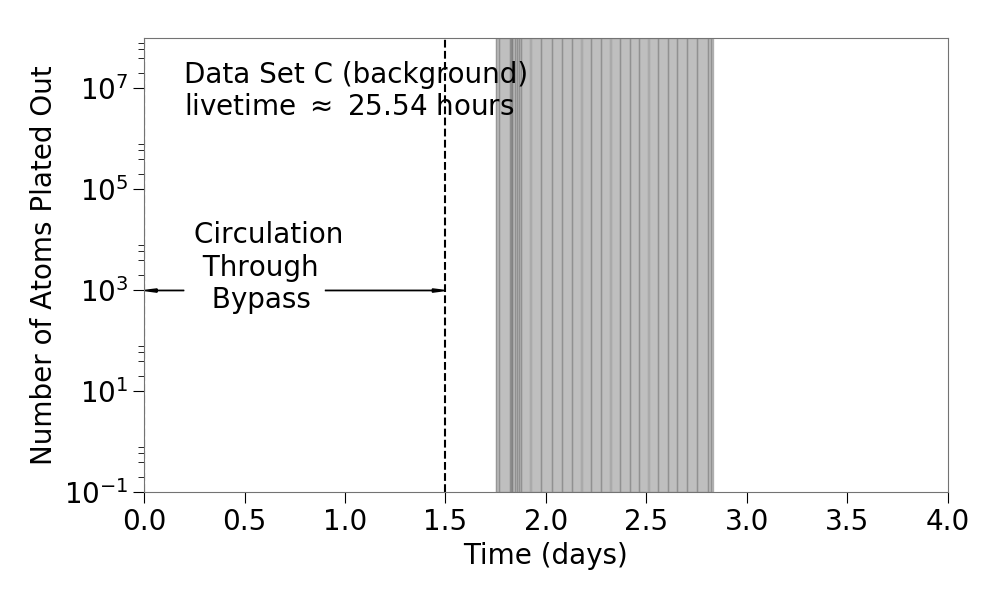
\includegraphics[width=\fullfig]{figures/radon/livetime_c.png}}
\caption{a) and (b) and (c) show the plateout conditions of datasets A, B, and C, respectively. The gray bands indicate time when data was being acquired. Dataset D (calibration) was taken following dataset A and consisted of a few hours.}
\label{fig:plate_out}
\end{figure}


%   \begin{figure}[ht]{0.6\textwidth}
%   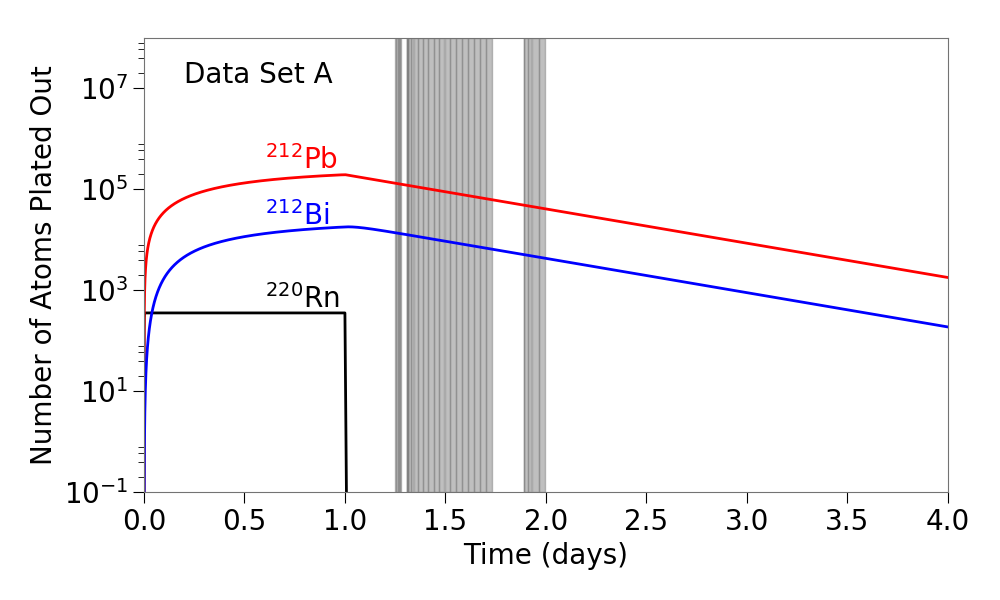
\includegraphics[width=1\linewidth]{figures/radon/livetime_a.png}
 %  \caption{}
 %  \label{fig:lt_a} 
%\end{figure}
%\begin{figure}[ht]{0.6\textwidth}
  % 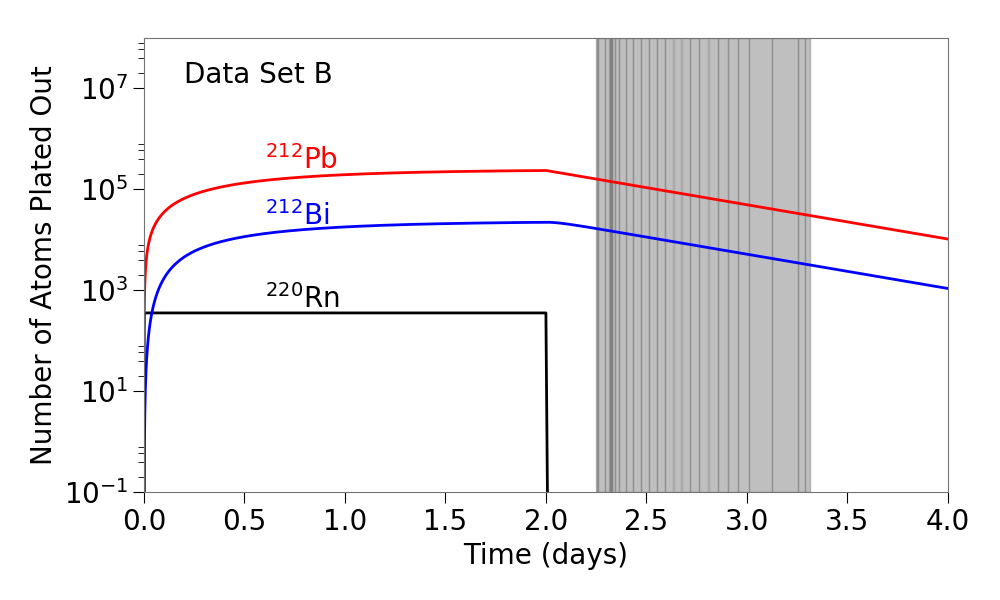
\includegraphics[width=1\linewidth]{figures/radon/livetime_b.png}
   %\caption{}
 %  \label{fig:lt_b}
%\end{figure}
%\begin{figure}[ht]{0.6\textwidth}
 %  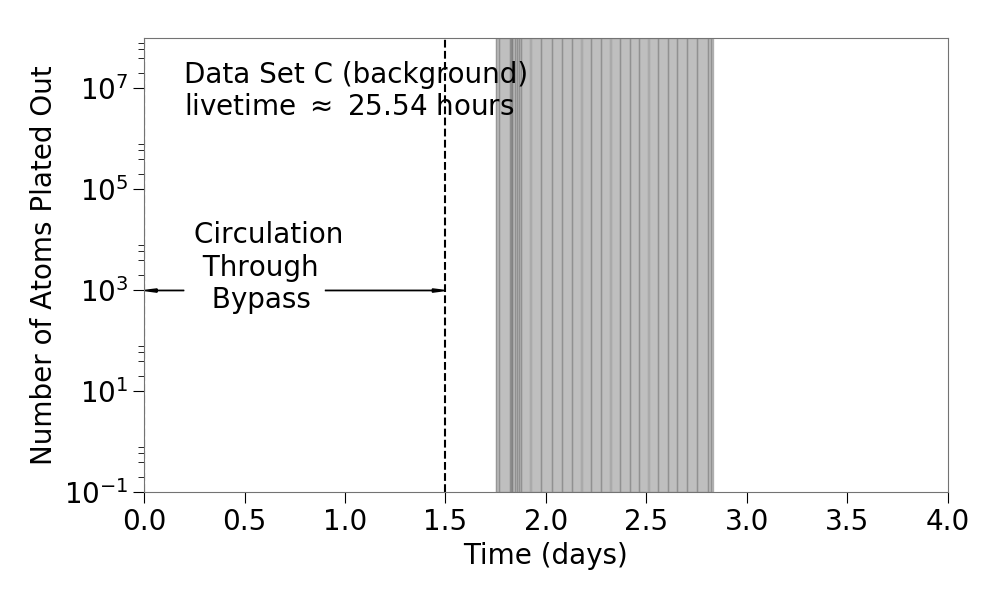
\includegraphics[width=1\linewidth]{figures/radon/livetime_c.png}
 %  \caption{}
  % \label{fig:lt_c}
%\end{figure}
%\caption[]{(a) and (b) and (c) show the plateout conditions of datasets A, B, and C, respectively. The gray bands indicate time when data was being acquired. Dataset D (calibration) was taken following dataset A and consisted of a few hours.}
%\label{fig:plate_out}
%\end{subfigures}



\subsection{Data Selection}
The trigger described in Sec. $\ref{datacollection}$ captured the slow chain decays as shown in Fig. $\ref{fig:Rn220}$. The $^{212}$Bi beta decay is followed by the 300~ns alpha decay of $^{212}$Po; these decays are referred to herein as``Bi-Po".

%\begin{table}[h]
%\centering
%\begin{tabular}{llll}
%\hline
%\\[-5pt]
%%& \multicolumn{3}{c}{\bf Datasets}\\[-5pt]
%\\[-5pt]
%Parent & Decay Mode & Energy / Endpoint & Half-Life\\
%\\[-5pt]
%\hline
%\\[-5pt]
%$^{212}$Pb & $\beta$ & 0.57~MeV & 10.6~h \\
%\multirow{2}{*}{$^{212}$Bi} & $\beta$ (0.64 BR) & 2.2~MeV & \multirow{2}{*}{61~min %} \\
%& $\alpha$ (0.36 BR) & 6.2~MeV & \\
%$^{212}$Po & $\alpha$ & 8.9~MeV & 200~ns \\
%$^{208}$Tl & $\beta$ & 1.8~MeV & 3.1~min \\
%\end{tabular}
%\caption{Events occurring in the TPC as a result of plate out.}
%\label{T:2}
%\end{table}


%$^{212}$Pb decay (0.57~MeV beta, half life 10.6~hours), $^{212}$Bi decay (0.36 branching to 6.2~MeV alpha or 0.64 branching to 2.2~MeV beta, half life 61~minutes),  $^{212}$Po decay (8.9~MeV alpha, half life 300~ns), and  $^{208}$Tl decay (1.8~MeV beta, half life 3.1~minutes). The $^{212}$Bi beta decay is followed by the $^{212}$Po alpha in the same 76~$\mu$s event window; these decays are referred to herein as "Bi-Po".


The aim of this analysis was to reconstruct the z-position of radon daughter alpha decays via the timing difference between the S1 and S2 of an event. Therefore, Bi-Po events were rejected, as the two S2s presented a timing ambiguity. The focus was instead on identifying $^{212}$Bi alpha decays. All events were expected to take place on detector surfaces, so $^{212}$Bi alpha decays in the drift region indicate mobility of plated-out daughters $^{212}$Pb and/or $^{212}$Bi; it was not possible to determine whether the original position was on the cathode wires, PTFE walls, or other detector surface.

%Because many of the events take place on the cathode grid wires, decreased light collection caused by the wires (shadowing) and high, non-uniform fields complicate the light and charge yields, and therefore accurate energy reconstruction of events on the cathode wires is is hampered (discussed further below). Therefore, b
The software cuts used to select $^{212}$Bi alphas are described below: 
\begin{enumerate}
\item \textbf{Data Cleaning} Remove events with any railed charge channel.
\item \textbf{Fiducialization} Require more signal in the central anode segment than the other two concentric anode segments.
\item \textbf{Select Alpha Events} The tallest pulse in an event was required to be an S1. Alphas are higher energy than the other decays in the $^{220}$Rn chain, and have a characteristically high light yield, so this cut is generous in keeping all alpha events.
\item \textbf{Reject Bi-Po Topology} Of the alpha events, those with one S1 and one S2 (single-scatter) were classified as $^{212}$Bi alpha. Events with two S1s (one of which is alpha-like), and one or two S2s were classified as Bi-Po.
\item \textbf{Reject Bi-Po Energy} There are two ways a Bi-Po event can mimic the topology of $^{212}$Bi alpha: (i) alpha decay was prompt and so the scintillation signals from the beta and alpha were combined into one large S1 (ii) the beta was ejected into the cathode wire and therefore there was no signal detectable from the beta. To robustly identify $^{212}$Bi, the alpha S1 areas of $^{212}$Bi alpha and Bi-Po events from Step 2 were histogrammed and fit with Gaussian functions. $^{212}$Bi alpha events were tightly selected with a high and low S1 area cut placed on single-scatter alpha events: anything above $(\mu - 3\sigma)_{Bi-Po}$ was considered a Bi-Po event and anything below $(\mu - 3\sigma)_{Bi-alpha}$ was considered a beta or gamma, and discarded (Fig. $\ref{fig:area_cut}$). It should be noted that this cut doesn't affect the signal region for $^{212}$Bi alpha in bulk; it affects the region for $^{212}$Bi alpha on the cathode. This cut is conservative in discarding Bi-Po events, as this leads to a more conservative fraction for dissolved fraction of $^{212}$Bi alphas.
%Note that this step is only necessary if one wishes to count the number of $^{212}$Bi alphas observed on the cathode, where decreased light collection and high, non-uniform fields complicate the light and charge yields (S1 and S2 pulse areas). In the bulk region, a $^{212}$Bi alpha is easily distinguishable from a Bi-Po event with a prompt alpha because they differ by almost 3.0~MeV in energy.
\item \textbf{Z-position Cut} Events in the cathode region were separated from events in the bulk region with a z-position cut (discussed further below).
\item \textbf{Bulk Signal Area Cut} Only $^{212}$Bi alpha tagged events which also fell in a signal region expected from calibration with the $^{220}$Rn flow though source (Fig. $\ref{fig:all_plots_CD}$h) were considered to be daughters which have dissolved.
\end{enumerate}



\begin{figure}[hbtp]
\centering
\subfloat[]{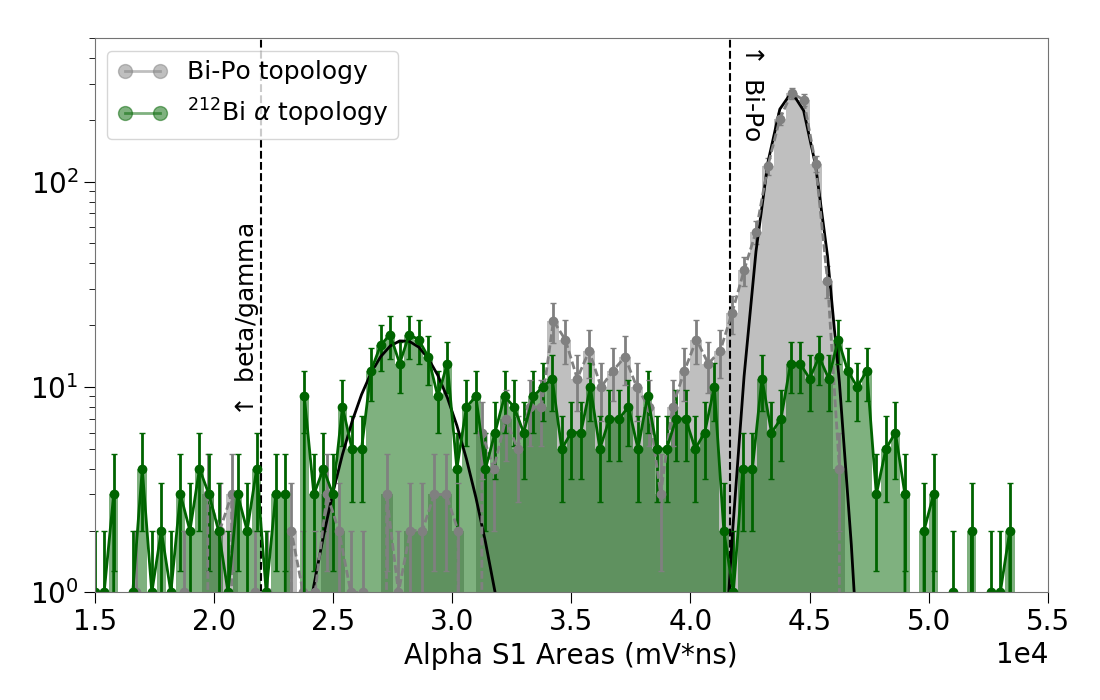
\includegraphics[width=\fullfig]{figures/radon/oct_alpha_s1_hist.png}}\\
\subfloat[]{ 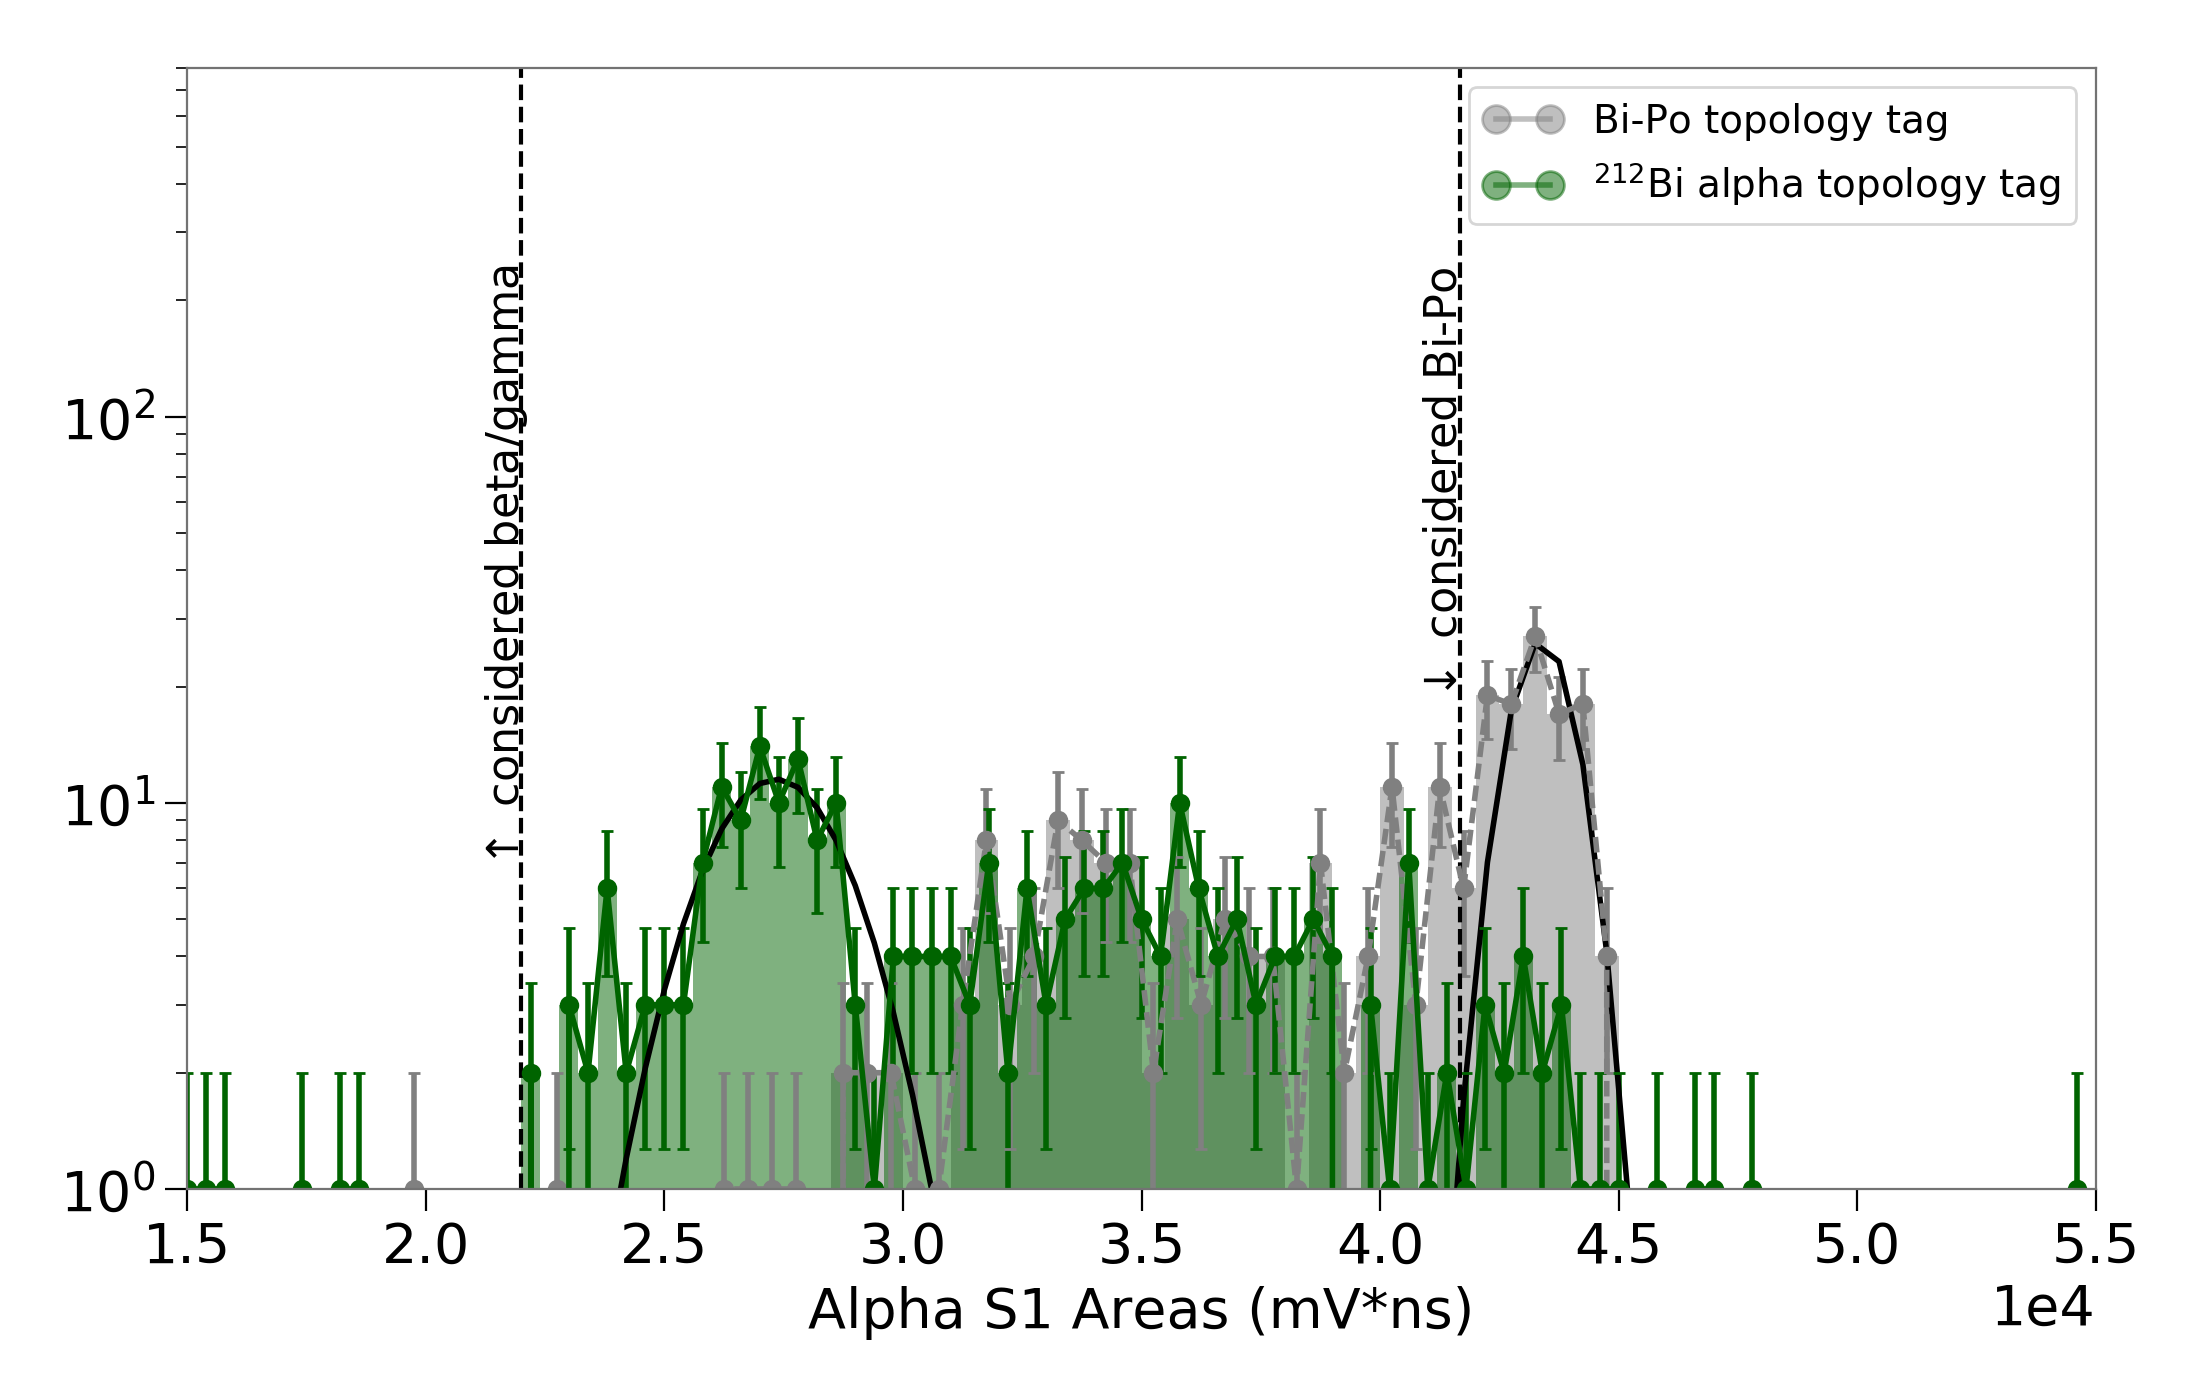
\includegraphics[width=\fullfig]{figures/radon/jan_alpha_s1_hist.png}}
\caption[]{The S1 areas of events that were tagged using topological features. These distributions were then used to employ the cuts in Step 3. The branching ratio for $^{212}Bi$ is 36:64 for $\alpha$:Bi-Po. Dataset (a) showed 10:90 and dataset (b) showed 35:65. It is unclear why the branching ratios for dataset (a) deviate so much from expectation. The trigger is more efficient for Bi-Po events because those decays would produce more a larger charge signal. It's possible that the cathode being left on during the plate out procedure had some effect on the geometrical distribution of daughters on the cathode wires, which further biased the trigger.}
\label{fig:area_cut}
\end{figure}


%\begin{figure}
%\centering
 %  \begin{subfigure}[ht]{0.6\textwidth}
%   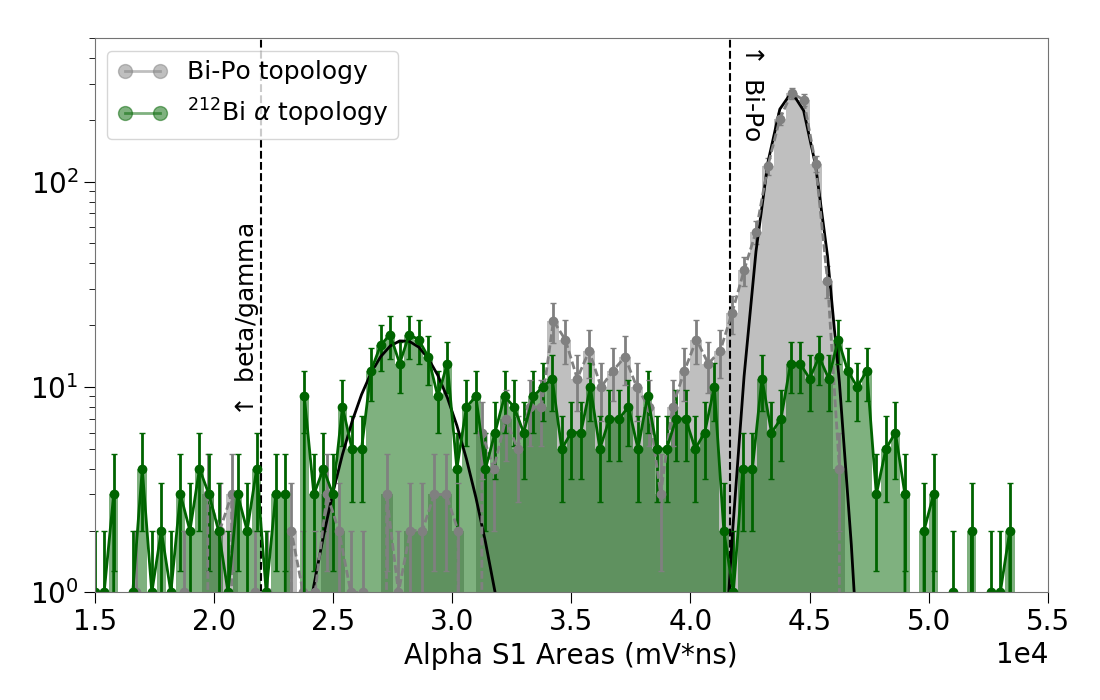
\includegraphics[width=1\linewidth]{figures/radon/oct_alpha_s1_hist.png}
%   \caption{}
 %  \label{fig:area_cut_a} 
%\end{subfigure}
%\begin{subfigure}[ht]{0.6\textwidth}
 %  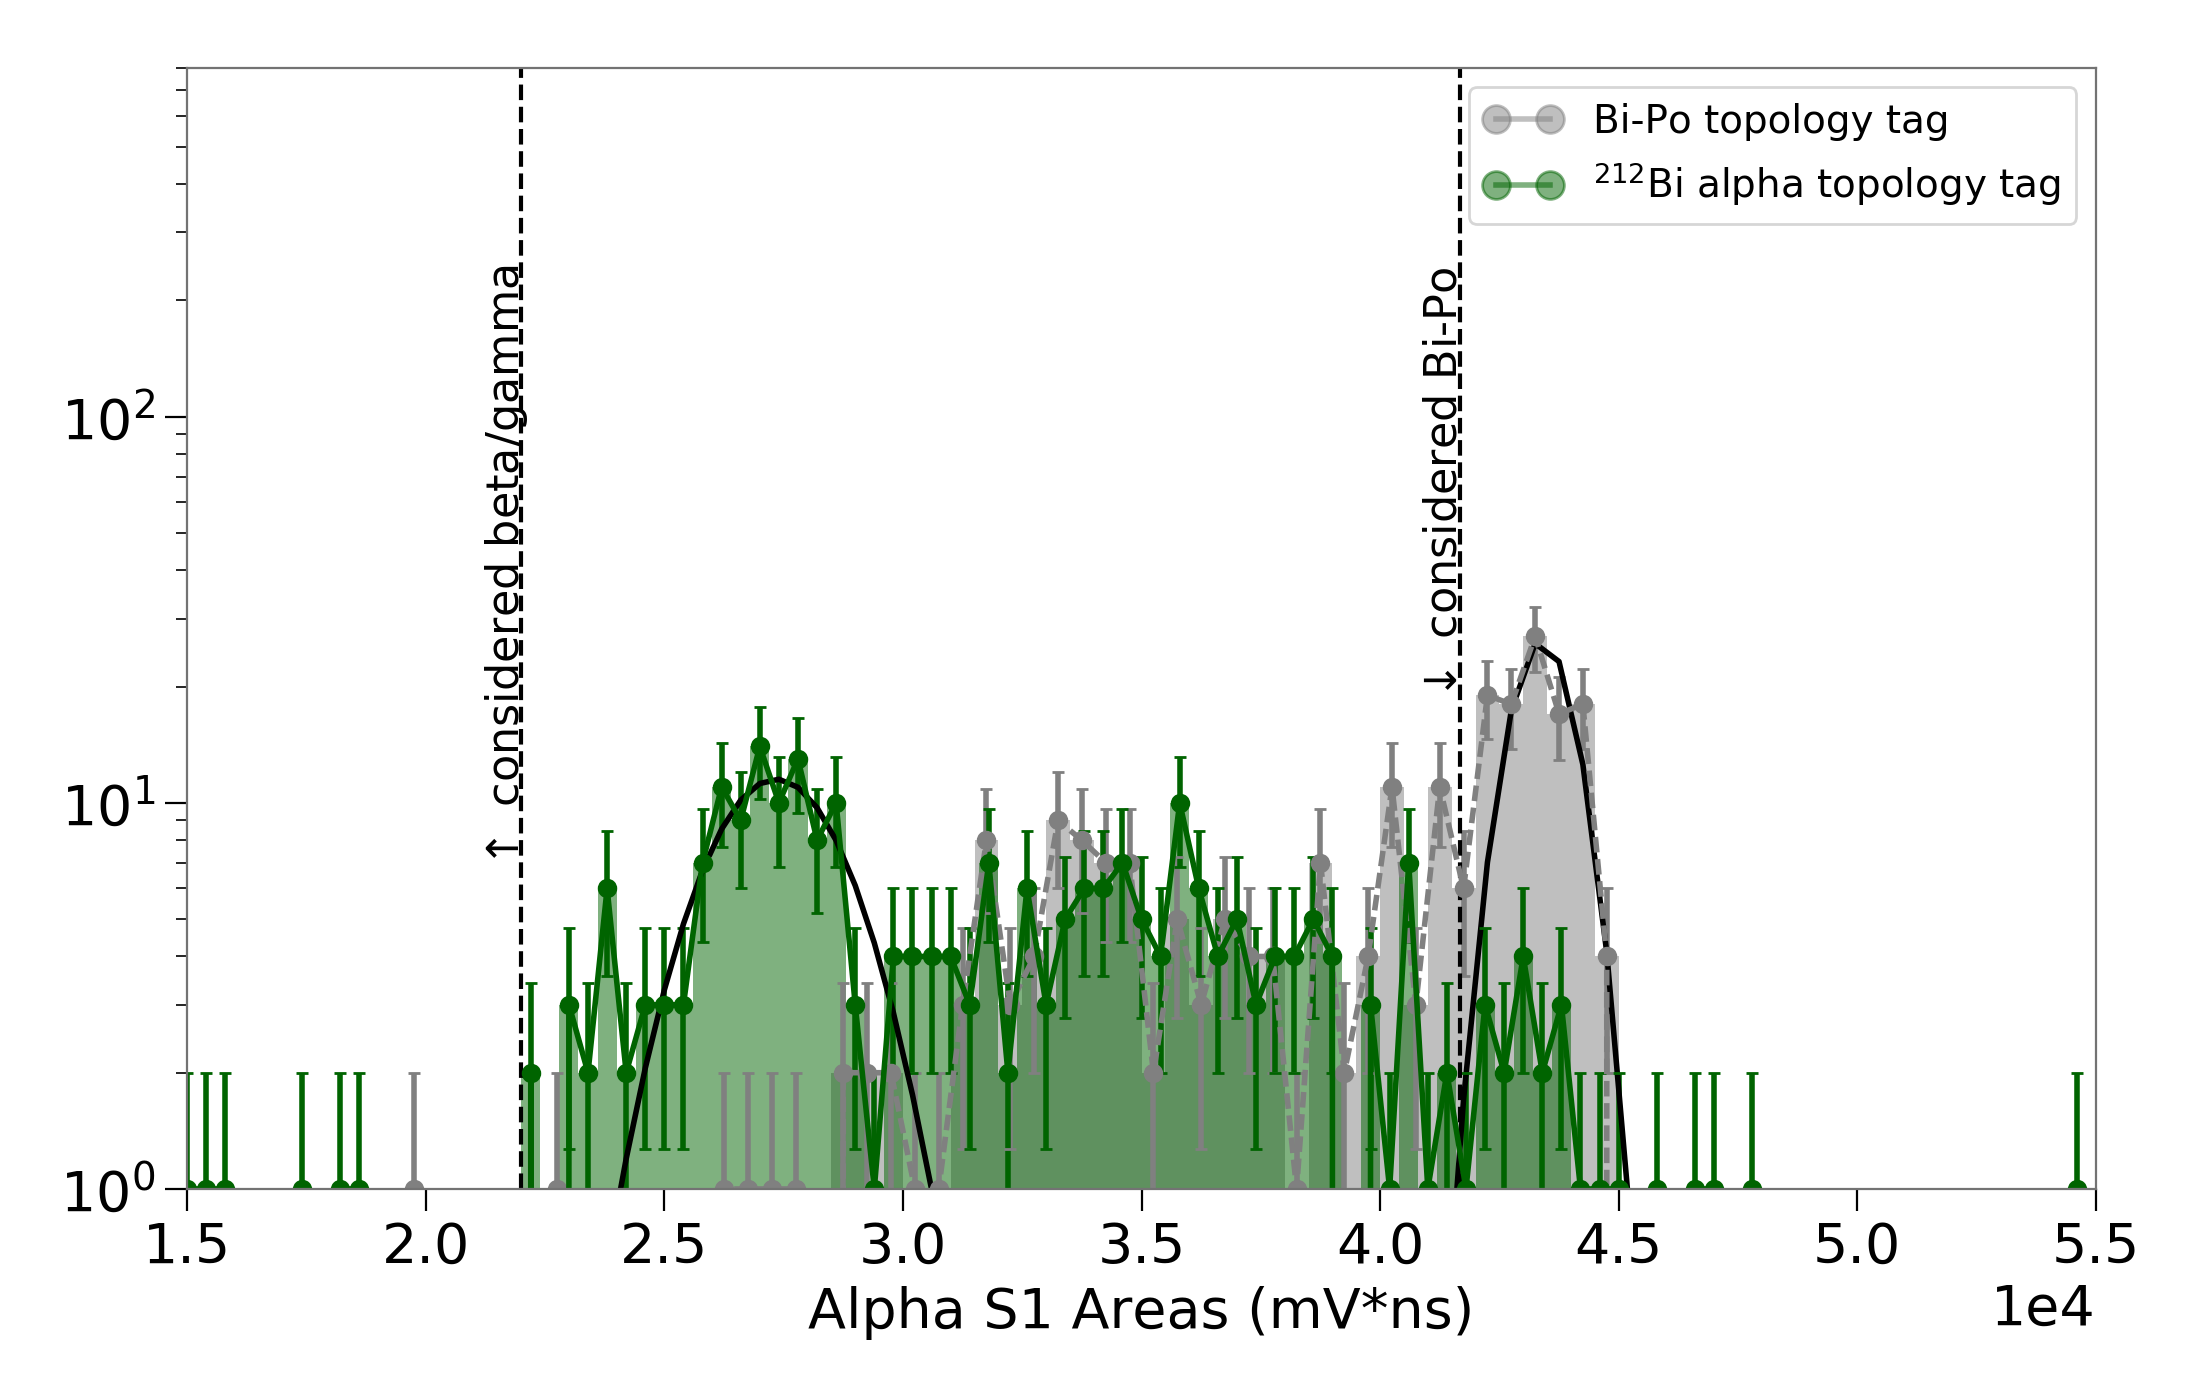
\includegraphics[width=1\linewidth]{figures/radon/jan_alpha_s1_hist.png}
  % \caption{}
 %  \label{fig:area_cut_b}
%\end{subfigure}
%\caption[]{The S1 areas of events that were tagged using topological features. These distributions were then used to employ the cuts in Step 3. The branching ratio for $^{212}Bi$ is 36:64 for $\alpha$:Bi-Po. Dataset (a) showed 10:90 and dataset (b) showed 35:65. It is unclear why the branching ratios for dataset (a) deviate so much from expectation. The trigger is more efficient for Bi-Po events because those decays would produce more a larger charge signal. It's possible that the cathode being left on during the plate out procedure had some effect on the geometrical distribution of daughters on the cathode wires, which further biased the trigger.}
%\label{fig:area_cut}
%\end{figure}


%Before any S1 and S2 pulse area event selection, event topology was used to classify events.  Of the alpha events, those with one S1 and one S2 (single-scatter) are classified as $^{212}$Bi alpha. Events with two S1s (one of which is alpha-like), and one or two S2s are classified as Bi-Po. The alpha S1 areas of $^{212}$Bi alpha and Bi-Po events are histogrammed and fit with Gaussian functions (show figure of this?). At this point, it is possible that some events tagged as $^{212}$Bi alpha are actually Bi-Po events where the alpha decay is prompt and so the scintillation signals from the beta and alpha are combined into one large S1, or the beta is ejected into the cathode wire and therefore there is no signal detectable from the beta. In order to tightly select $^{212}$Bi alpha events, a high and low S1 area cut is placed on single-scatter alpha events: anything above $\mu_{Bi-Po} - 3\sigma_{Bi-Po}$ is considered a Bi-Po event and anything below $\mu_{Bi-alpha} - 3\sigma_{Bi-alpha}$ is considered a beta or gamma. Events in the cathode region are separated from events in the bulk region with a z-position cut (discussed below). These event topology and S1 area cuts and z-position cuts are as robust as the recombination physics allows for classifying $^{212}$Bi alpha and Bi-Po events on the cathode. In the bulk, a $^{212}$Bi alpha is easily distinguishable from a Bi-Po event with a prompt alpha because they differ by almost 3.0~MeV in energy. The unique light collection and recombination effects of the cathode make tagging difficult in the cathode region only. In order to avoid any other ambiguity for signal events ($^{212}$Bi alpha in the bulk region), only $^{212}$Bi alpha tagged events which also fall in a signal region expected from calibration with the $^{220}$Rn flow though source (Fig. $\ref{fig:signalregion_calib}$) are considered to be daughters which have dissolved.

%We focus on a search for $^{212}$Bi alpha decays. Because many of the events take place on the cathode grid wires, shadowing and high, non-uniform fields complicate the light and charge yields, and therefore accurate energy reconstruction of events on the cathode wires is is hampered. Therefore, before any S1 and S2 pulse area event selection, event topology is used to select candidate $^{212}$Bi alpha events. The simplest cut, which selects alpha events, requires the tallest pulse in an event to be an S1 and requires it to fall in a tight prompt fraction-pulse width region (show a figure of this?). Since alphas are known for their characteristic recombination with high (90\%) light yield only weakly dependent on field, this is more than generous in keeping all alpha events. Contamination from betas and gammas is possible, but unlikely. The second event topology cut requires only one S1 and one S2 in the event window, this cuts multi-scatter beta and gamma events as well as Bi-Po events. Events in the cathode region are separated from events in the bulk region with a z-position cut (see below for how this z is chosen). These event topology cuts and z-position cuts leave four possible event types that could mimic a $^{212}$Bi alpha decay in the bulk region:

%\begin{enumerate}
%\item Cathode single scatter beta or gamma interactions mis-tagged as alphas (rare), with beta or gamma penetrating into the bulk region.
%\item Bulk single scatter beta or gamma interactions mis-tagged as alphas (rare).
%\item Overlapping Bi-Po in bulk region. This is where the $^{212}$Po alpha immediately follows the $^{212}$Bi beta, such that only one large (alpha-like) S1 appears. 
%\item Overlapping Bi-Po on cathode wire, with beta penetrating into the bulk region, thereby appearing to be a bulk event. 
%\end{enumerate}

%Events of types 2 and 3 are excluded by only choosing $^{212}$Bi alpha bulk events which fall within a signal region determined from calibration with the flow through source (Fig. $\ref{fig:signalregion_calib}$). Events of types 1 and 4 are excluded with the choice of $z$ that defines the cathode region from the bulk region. 

In order to choose the value for the z-position cut in Step 4, a Monte Carlo approach was used. A Bi-Po decay with a prompt alpha (appears as single-scatter) where the beta penetrates into the bulk region, could mimic a $^{212}$Bi alpha bulk event. To better understand Bi-Po cathode events and the danger of mis-identifying them as $^{212}$Bi alphas in bulk, a Monte Carlo study was done with the $^{212}$Bi beta spectrum (the highest energy beta in the $^{220}$Rn chain) to determine the maximum distance a beta could penetrate into the bulk region. The study yielded a maximum beta penetration of $zmax_{MC}$ = 0.12~cm, see Fig. $\ref{fig:betaMC}$. 
The $z$ position cut separating cathode from bulk was then defined to be $z_{cut} = zmax_{MC} + 3\sigma_{fit}$, where $\sigma_{fit}$ is just the width of a Gaussian fit for the position of the cathode. Figures $\ref{fig:all_plots_AB}$a and $\ref{fig:all_plots_AB}$c show the cathode position fits as well the the location of $z_{cut}$. The cathode position fit error, $\sigma_{fit}$, was the same for both datasets A and B, and was also used to determine $z_{cut}$ for the background and calibration sets.

%events are particularly easy to select because of the large S1, so we focus on a search for $^{212}$Bi in bulk.  $^{212}$Bi has a 0.36 branching ratio to a 6.2~MeV alpha and 0.64 branching ratio to a 2.9~MeV beta which is followed by the fast decay of $^{212}$Po via an 8.9~MeV alpha. This beta-alpha, referred to herein as "Bi-Po", occurs in the same event window
%This analysis reconstructs the z-position of $^{212}$Bi decays via the timing difference between the S1 and S2 of an event. Therefore, we reject BiPo events, the two S2s present a timing ambiguity. We expect all events to take place on the cathode; $^{212}$Bi alpha decays in the drift region indicate mobility of plated-out daughters $^{212}Pb$ and/or $^{212}$Bi.
%Sources of events that could mimic a $^{212}$Bi drift region event are
%(a) On the cathode: BiPo event with a prompt $^{212}$Po decay such that the beta S1 and alpha S1 (as well as their S2s) overlap. -- okay because we cut far enough away that the beta won't mimic 
%(b) The situation in (a) occurring in the drift region.
%0.57~MeV betas from $^{212}$Pb decay, 6.2~MeV alphas from one branch of $^{212}$Bi decay (0.36 brancing ratio), where the other branch (referred to as "Bi-Po") results in 2.9~MeV beta followed within the event window by a 8.9~MeV $^{212}$Po alpha. There is also a 1.8~MeV beta from $^{208}$Tl decay. Because many of the events take place on the cathode grid wires, shadowing and high, non-uniform fields complicate the light and charge yields, and therefore accurate energy reconstruction is is hampered. Before any energy-based event selection, event topology is used to select $^{212}$Bi alpha events. Bi-Po (beta-alpha) events are rejected for this analysis because the beta complicates z-position reconstruction.
%Most BiPo events can be cut via coincidence tagging, however, in the case of a prompt $^{212}$Po decay, PMT signals for the beta S1 and alpha S1 (as well as their S2s) could overlap, mimicking a $^{212}$Bi alpha decay. If these "fake" $^{212}$Bi alpha events were to happen in the drift region, the energy of the 8.9~MeV alpha would clearly identify it from the 6.2~MeV alpha. However, on the cathode, the unusual recombination could cause a mis-identification. This situation is of concern because betas travel further in liquid xenon that do alphas. Therefore, a Monte Carlo study was done for the $^{212}$Bi beta decay spectrum to determine the maximum depth into the drift region a beta on the cathode could penetrate (Fig. $\ref{fig:betaMC}$). The study selected an energy from the $^{212}$Bi beta spectrum (from IAEA), found the CDSA range for a beta of that energy (NIST), and then translated the CDSA range to actual depth by the method in Tabata (ref). The farthest such a beta could be expected to travel was found to be 0.12cm (0.6~us). Since the drift region of the detector measures 1.0~cm (6us) in depth, errant betas from the cathode do not pose a risk to the analysis.

\begin{figure}[ht]
    \centering
    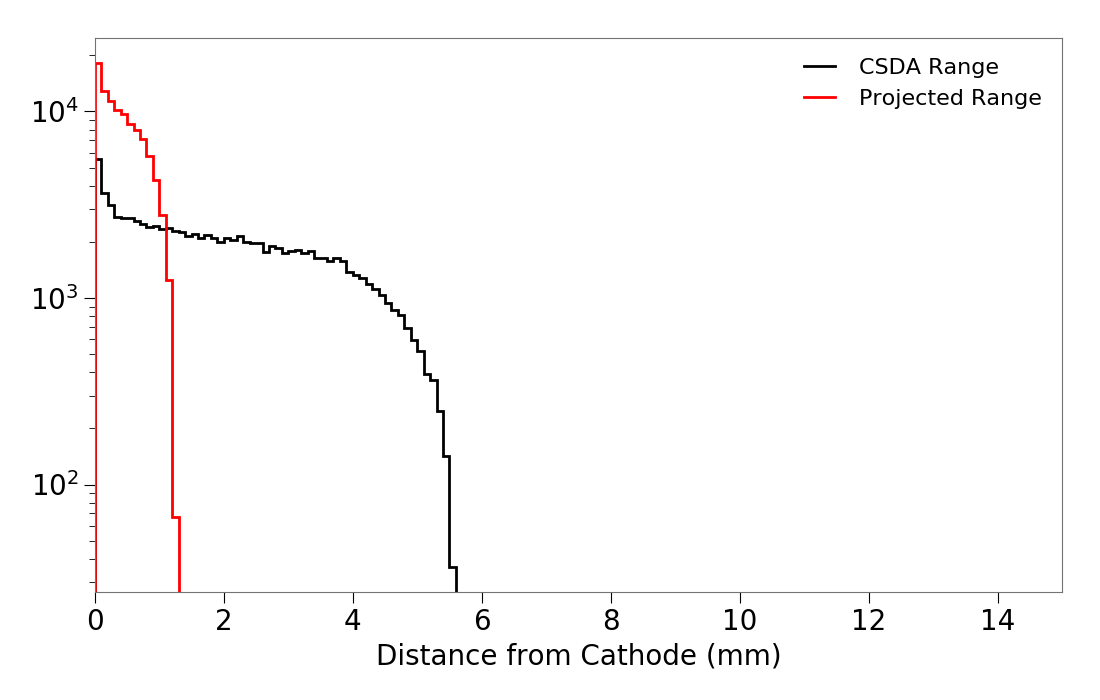
\includegraphics[width=3in]{figures/radon/betaMC_ranges_logy.png}
    \caption{Monte Carlo study to find the maximum distance a $^{212}$Bi beta (2.2~MeV) on the cathode could penetrate into the drift region. The projected range (red) is the relevant curve for this analysis; it shows a beta is not expected to travel more than 1.2mm from the cathode.}
    \label{fig:betaMC}
\end{figure}




\begin{figure}[hbtp]
\centering
\rotatebox[origin=b]{90}{Dataset A}\subfloat[]{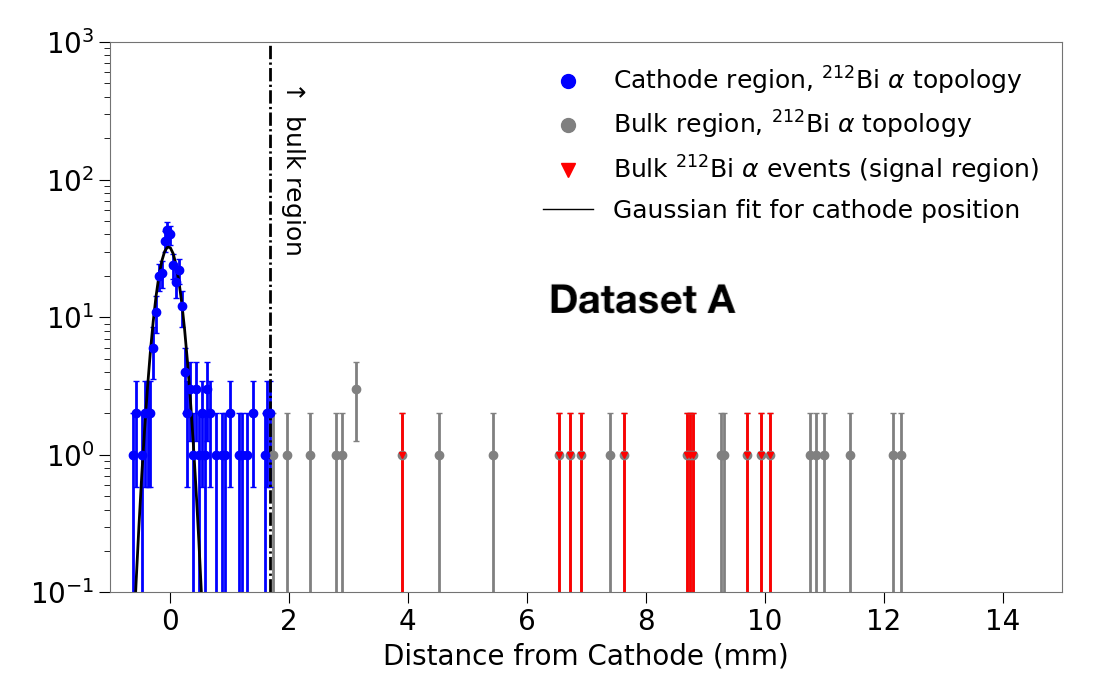
\includegraphics[width=0.6\textwidth]{figures/radon/hist_a.png}} \subfloat[]{ 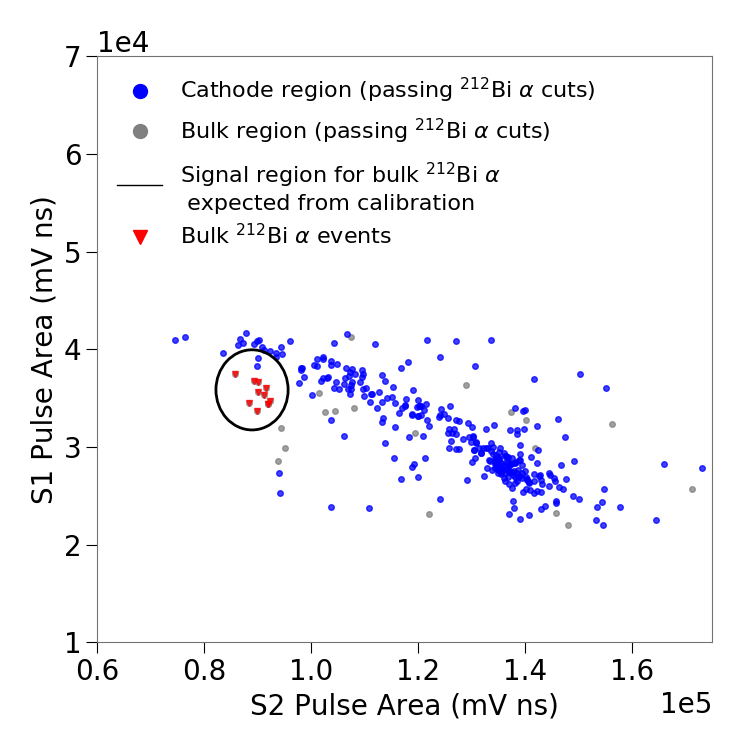
\includegraphics[width=0.4\textwidth]{figures/radon/signalregion_a.png}}\\
\rotatebox[origin=b]{90}{Dataset B}\subfloat[]{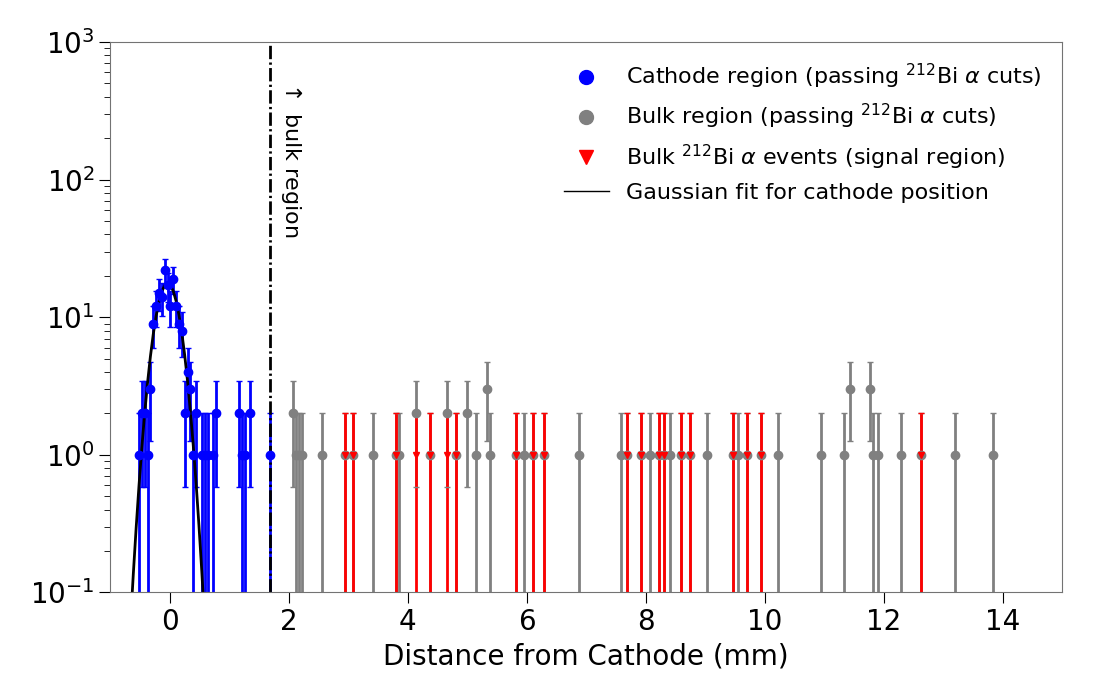
\includegraphics[width=0.6\textwidth]{figures/radon/hist_b.png}} \subfloat[]{ 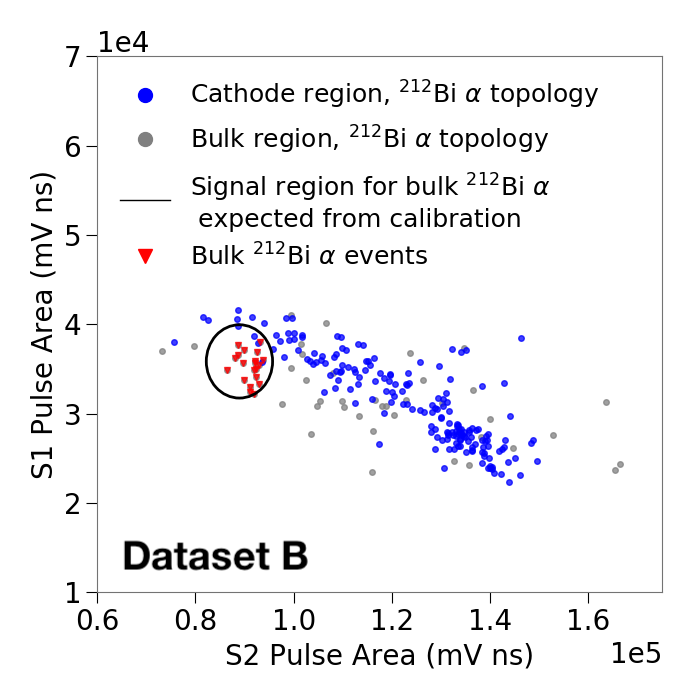
\includegraphics[width=0.4\textwidth]{figures/radon/signalregion_b.png}}\\
\caption{For datasets A and B: \textbf{(left)} Distribution of events in $z$. \textbf{(right)}  The same events distributed in the S1-S2 plane, showing selection criteria for candidate $^{212}$Bi alpha events in the bulk liquid xenon.} 
\label{fig:all_plots_AB}
\end{figure}

\begin{figure}[hbtp]
\centering
\rotatebox[origin=b]{90}{Dataset C}\subfloat[]{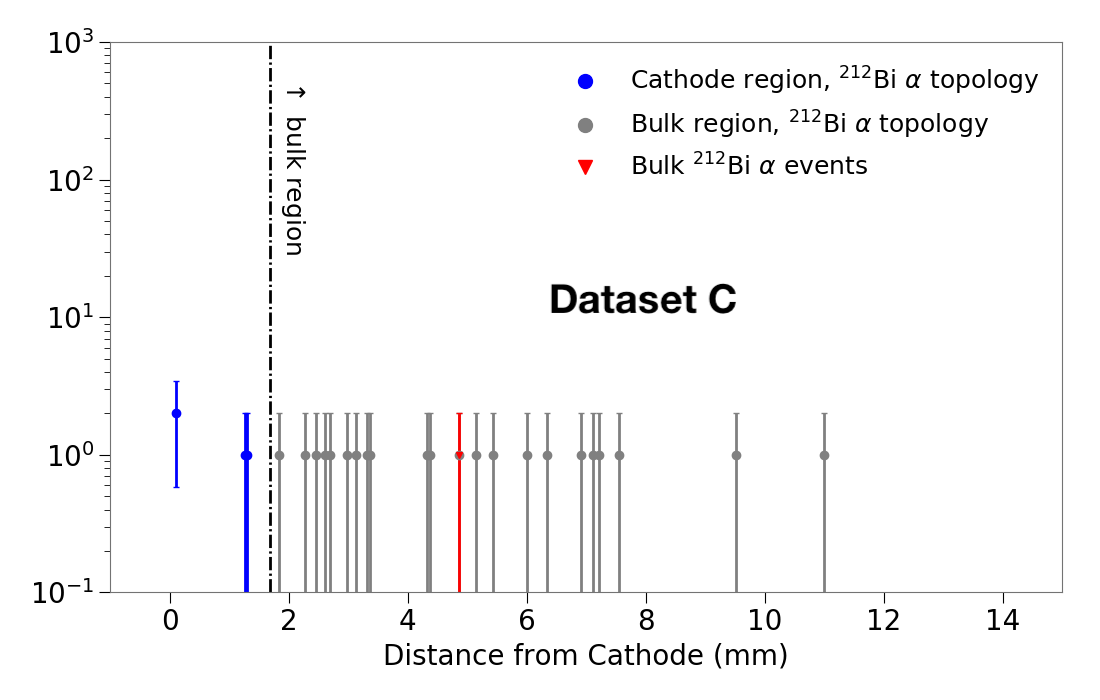
\includegraphics[width=0.6\textwidth]{figures/radon/hist_bkg.png}} \subfloat[]{ 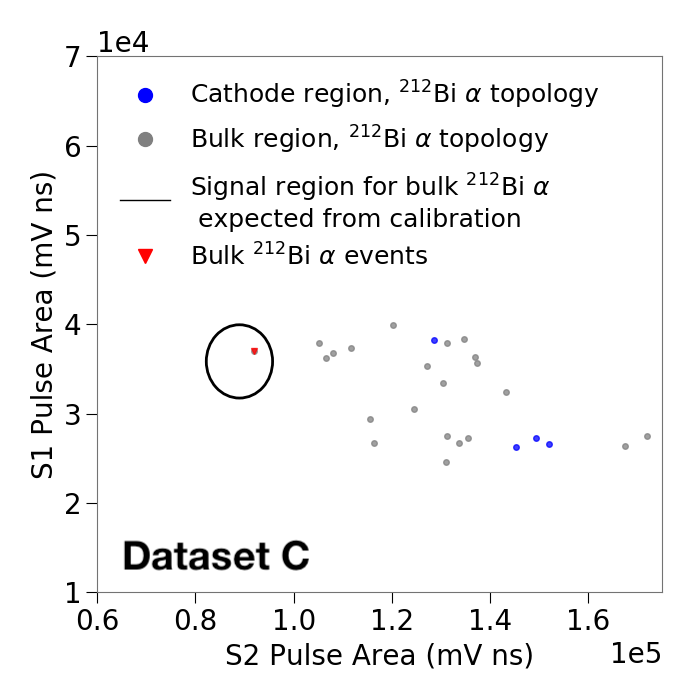
\includegraphics[width=0.4\textwidth]{figures/radon/signalregion_bkg.png}}\\
\rotatebox[origin=b]{90}{Dataset D}\subfloat[]{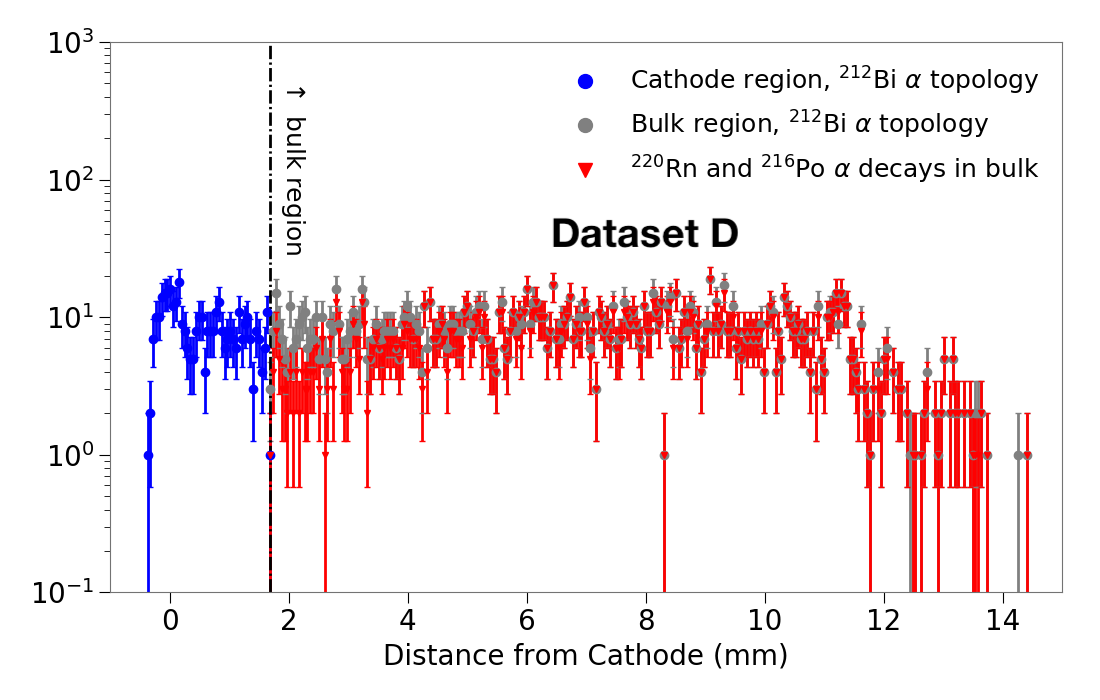
\includegraphics[width=0.6\textwidth]{figures/radon/hist_calib.png}} \subfloat[]{ 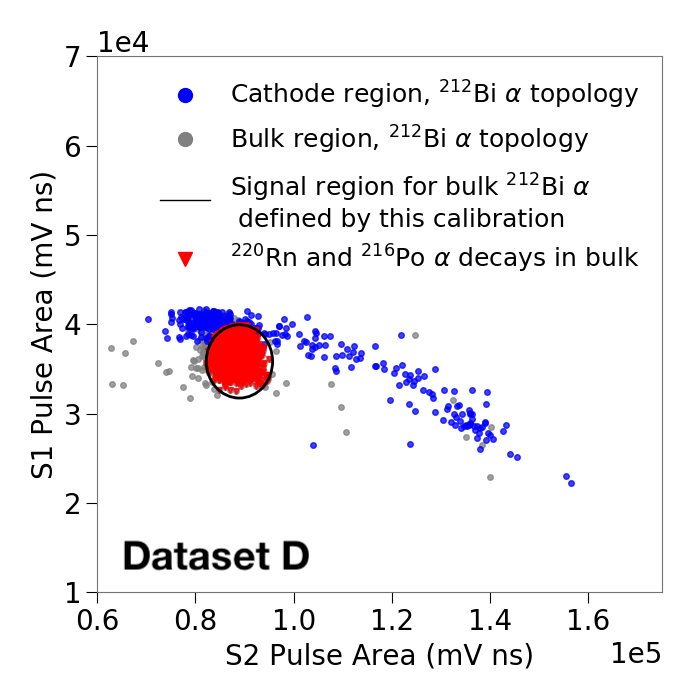
\includegraphics[width=0.4\textwidth]{figures/radon/signalregion_calib.png}}\\
\caption{For datasets C and D: \textbf{(left)} Distribution of events in $z$. \textbf{(right)}  The same events distributed in the S1-S2 plane, showing selection criteria for candidate $^{212}$Bi alpha events in the bulk liquid xenon.} 
\label{fig:all_plots_CD}
\end{figure}


One feature that merits further discussion from Figure $\ref{fig:all_plots_AB}$ is the strong anti-correlation in S1 Pulse Area vs. S2 Pulse Area apparent in cathode events. The cathode region was subject to very high, non-uniform fields due to the thin wires that comprised the cathode grid. Events that occurred on the wires encountered different fields depending on their position on the surface of the wire. Additionally, two events that occurred at exactly the same spot encountered different fields depending on which direction the decay particle (alpha, beta, etc.) traveled. The amount of scintillation and ionization from an interaction in liquid xenon depends on the field at the interaction site. Higher fields result in more ionization electrons being separated from the interaction site and therefore more S2. Mono-energetic events occurring in a uniform field have small anti-correlated fluctuations in S1 and S2 size. Non-uniform fields greatly exaggerate the typical variation in S1 and S2 size resulting in the spread out cathode region (blue) observed in Figures $\ref{fig:all_plots_AB}$ and $\ref{fig:all_plots_CD}$  (right). Events in the bulk region encounter a relatively low, uniform field resulting in a compact signal region in S1 vs. S2 (visible in red region of calibration data, Dataset D). 

%Some interesting differences between dataset A and B stems from the plate out conditions. Dataset A has a clear beta tail coming off the cathode -- these are Bi-Po events occurring on the cathode, where the beta has penetrated the bulk region, thereby artificially decreasing the time between the alpha S1 and subsequent S2. The more prevalent beta tail can be attributed to the cathode preferentially collecting daughters in the plate-out stage in dataset A due to a supplied voltage. It is interesting to note that for dataset B there are many events events still originate from the cathode, which may indicate a migration of daughters from initial positions on the PTFE walls towards the cathode. 

\section{Results and Discussion}
\label{results}
We observed 11 bulk $^{212}$Bi alphas for dataset A, 20 for dataset B, and 1 background event in the signal region from dataset C. The counts of cathode region $^{212}$Bi alphas are presented in Table $\ref{T:3}$. There was only one background event observed in the signal region, so with 95\% confidence the true background count is at most 4.74. The observed counts for dataset A and B lie far above the 95\% confidence limit for background, indicating they are true observations of  $^{212}$Bi alphas in bulk. Defining dissolved fraction as $N_{bulk}$ / $N_{cath}$, the dissolved fraction of $^{212}$Bi alphas for dataset A ($\approx$ 13~h livetime) is 0.035 $\pm$ 0.010, and for data set B ($\approx$ 25~h livetime) is 0.099 $\pm$ 0.020. 

These results indicate that either $^{212}$Pb or $^{212}$Bi itself is soluble to a small degree in liquid xenon. 

%Furthermore, the dissolved fraction per livetime for data set A being less than that of data set B may indicate that daughters adsorbed on Teflon are more likely to dissolve than daughters adsorbed on stainless steel. The rate of $^{220}$Rn entering the detector during the plate-out step was the same for both datasets A and B, but for data set A charged daughters were attracted preferentially to the cathode.
%The 95\% confidence intervals for dataset A (observed 11 counts) are [4.50, 17.50] and dataset B (observed 20 counts) are [11.23,28.76] 

%Findings are consistent with LUX: migration of daughters to cathode and also no large solubility of plated-out daughters into bulk region (LUX bulk >> test bed bulk).  (I don't think this is published yet? Kelsey is currently working on finding radon daughter dissolved events in the bulk.) However, in a field where the signal would be on the order of a few events, a few events of soluble radon should be included in background models.

\begin{table}[ht]
\centering
\caption{Number of detected alpha particle events whose energy determination was consistent with $^{212}$Bi decay to $^{208}$Tl. Live times are quoted in Table $\ref{T:1}$}
\begin{tabular}{llccc}
\hline
\\[-5pt]
%& \multicolumn{3}{c}{\bf Datasets}\\[-5pt]
%\\[-5pt]
dataset ID: & A &B & C \\
%\\[-5pt]
\hline
\\[-5pt]

Bulk Events & 11 & 20 & 1 \\
Cathode Events & 300 & 183 & 4 \\
%& Dissolved Fraction of $^{212}$Bi $\alpha$ & 0.035 $\pm$ 0.010 & 0.099 $\pm$ 0.020 & 0.02 $\pm$ 0.18  \\
%quote in results section
\\[-5pt]

\\[-5pt]

\hline
\end{tabular}
\label{T:3}
\end{table}



The solubility is presented in the following units:

%\centering
\begin{equation*}
\centering
$$
\frac{\displaystyle  \frac{\displaystyle Bq~(dissolved)}{\displaystyle kg~LXe} }{\displaystyle  \frac{\displaystyle Bq~(plated~out)}{\displaystyle cm^{2}~(detector~surface)} }
$$
\end{equation*}



\begin{table}[ht]
\centering
\caption{Using observations from $\ref{T:3}$, proceed through solubility calculation.}
\begin{tabular}{lcc}
\hline
\\[-5pt]
%& \multicolumn{3}{c}{\bf Datasets}\\[-5pt]
%\\[-5pt]
dataset ID: & A &B \\
%\\[-5pt]
\hline
\\[-5pt]
Total Inferred Bi decays & 20 $\pm$ 6 & 36 $\pm$ 11 \\
Livetime (hours) & 12.02 $\pm$ 0.5 & 23.93 $\pm$ 0.5 \\
$\mu$Bq Bi in bulk & 460 $\pm$ 140 &  420 $\pm$ 130 \\
Bq (dissolved) / kg LXe (smallest fiducial) & 0.42 $\pm$ 0.13 & 0.38 $\pm$ 0.12 \\
Bq (dissolved) / kg LXe (largest fiducial) & 0.0063 $\pm$ 0.0020  &  0.0057 $\pm$ 0.0018\\
\hline \\
\multicolumn{3}{c}{Plate-Out Areas} \\
\hline
 & Area \\
Total Internal Area Including PMT & 496 cm$^{2}$ \\ % & 1 \\
Active Region PTFE & 36 cm$^{2}$ \\ % & 0.07 \\
%Full Interior Region PTFE & 295 cm$^{2}$ & 0.6 \\
\hline \\
dataset ID: & A &B \\
Number of $^{212}$Bi Plated-Out & 13191  & 17280 \\
Bq (plated-out) & 2.5  & 3.2 \\
%\hline \\
%Number of $^{212}$Bi on All PTFE & 7914 & 10368 \\
%Bq (plated-out)  & 1.5 & 2.0  \\
%\hline \\
%Number of $^{212}$Bi on Active PTFE & 923 & 1209 \\
%Bq (plated-out)  & 0.17 & 0.23 \\
\hline \\
Bq (plated) / cm$^{2}$ min & 0.0050  $\pm$ 0.0005  & 0.0065  $\pm$ 0.0007\\
Bq (plated) / cm$^{2}$ max & 0.069  $\pm$ 0.007 & 0.089  $\pm$ 0.009  \\
\hline
\multicolumn{3}{c}{Solubility} \\
\hline
dataset ID: & A &B \\
Solubility min & 0.091 $\pm$ 0.030 & 0.064 $\pm$ 0.021\\
Solubility max & 84. $\pm$ 26. & 58. $\pm$ 18. \\

%& Dissolved Fraction of $^{212}$Bi $\alpha$ & 0.035 $\pm$ 0.010 & 0.099 $\pm$ 0.020 & 0.02 $\pm$ 0.18  \\
%quote in results section
\\[-5pt]

\\[-5pt]

\hline
\end{tabular}
\label{T:solubility}
\end{table}


The solubility calculation is subject to errors from the following factors. Where appropriate, it is noted how the error taken into account in the calculation; otherwise, the assumption is stated.
\begin{enumerate}
\item Liquid height (folded into fiducial volume)
\item Area over which charge amps are sensitive (calculation using different fiducial volumes)
\item Area over which daughters are plated out (varying area over which $^{212}$Bi is distributed; assume 10\% error in area calculation)
\item Initial activity of plated out daughters (assume circulation time for gas to leave inner PTFE stack > decay time of $^{216}$Po)
\item Live time calculation (uncertainty included)
\end{enumerate}

The solubility found in dataset A is at worst 84 $\pm$ 26 Bq/kg/Bq/cm$^{2}$ and at best 0.091 $\pm$ 0.030 Bq/kg/Bq/cm$^{2}$. For dataset B, the worst case is 58. $\pm$ 18. Bq/kg/Bq/cm$^{2}$ and the best case is 0.064 $\pm$ 0.021 Bq/kg/Bq/cm$^{2}$. 

These results are first evidence that the $^{220}$Rn daughters $^{212}$Pb and/or $^{212}$Bi are soluble in liquid xenon. The dissolved events are a small fraction of events that are plated-out on detector surfaces. These daughters are proxies for the isotopes $^{210}$Pb and/or $^{210}$Bi, which undergo naked beta decays in the $^{222}$Rn chain and pose a problem for liquid xenon dark matter detectors. Our study counts dissolved $^{212}$Bi alpha events as well as $^{212}$Bi alphas plated out on the cathode. We found 11 counts in dataset A and 20 counts in dataset B consistent with $^{212}$Bi decay in the bulk region; these counts are significantly above a background count of 1. The experimental apparatus is not characterized extensively. Regardless, we carried through the solubility calculation, taking into account uncertainties to arrive at a `best case' and `worst case' result. 

The limit derived from LUX observations, stated in the LZ projected sensitivity paper \cite{LZ:Sensitivity}, is 0.1~$\mu$~Bq/kg LXe for $^{212}$Bi mobility, given 50~nBq/cm$^{2}$ on PTFE panels. Our observed solubility is much greater than this. One explanation is that we are sensitive to the `stuck' radon daughters that wash off easily in the first few days of an experiment due to the introduction of \ac{LXe}. Large TPCs may then expect an increased rate of radon daughter decays in the fiducial volume at the beginning of a search, but a decreasing rate as these are removed by the getter or are implanted in detector materials. 

Another, testable, explanation that would reconcile the different solubilities in the $^{220}$Rn and $^{222}$Rn chain is beta ejection. Referring to Figures $\ref{Rn220}$ and $\ref{Rn222}$, both bottleneck decays, $^{XXX}$Pb, are beta decays. However, $^{212}$Pb in the $^{220}$Rn chain has a beta decay endpoint of 570~keV, which about 10 times of the endpoint energy for $^{210}$Pb in the $^{222}$Rn chain. Daughter recoils from beta decay are indeed small; the endpoints are approximately 0.6~eV for the recoil from $^{212}$Pb decay in the $^{220}$Rn chain and  0.006~eV for the recoil from $^{210}Pb$ decay in the $^{222}$Rn chain. The physisorption potential in for both cases is expected to be below 1~eV. Depending on the exact value, which is unavailable, the $^{212}$Pb decay could provide enough energy to liberate the daughter $^{212}$Bi most of the time, where as $^{210}$Pb decay produces a maximum recoil value below the potential depth. 

Further study, where a known amount of $^{220}$Rn daughters are plated out on a known area is necessary to measure dissolution rates. Additional studies that compare the solubility of radon daughters adsorbed on different materials, and under different conditions (e.g. temperature) would also be useful. The effect of cleaning these surfaces before searching for dissolved daughters should also be investigated. 

If beta recoil, not `washing' by the \ac{LXe}, is the cause of radon daughter solubility, then the high rate seen by this study of $^{220}$Rn can be reconciled with the low rate of $^{222}$Rn  daughter dissolution seen in large experiments.


%*****************************************
%*****************************************
%*****************************************
%*****************************************
%*****************************************
